\chapter{Implementation} \label{implementation}

Die Implementation hat zum Ziel, die bereits erarbeitete konzeptionelle Lösung in Form von Code praktisch umzusetzen. Nach einer Übersicht über die abgeschlossene Visualisierung und einem Einblick in die eingesetzten Technologien wird im Detail auf nennenswerte Eigenheiten des Projektes eingegangen.

\section{Übersicht}
Nachfolgend ist die integrierte Visualisierung innerhalb des \gls{ikc-core}[s] ersichtlich (\autoref{fig:overview-implementation}). Sie wurde zwischen der Suche und der Detail-Ansicht platziert. Eine detaillierte Anleitung der Interaktion mit der integrierten Visualisierung ist dem Benutzerhandbuch zu entnehmen. 

\begin{figure}[htbp]
\centerline{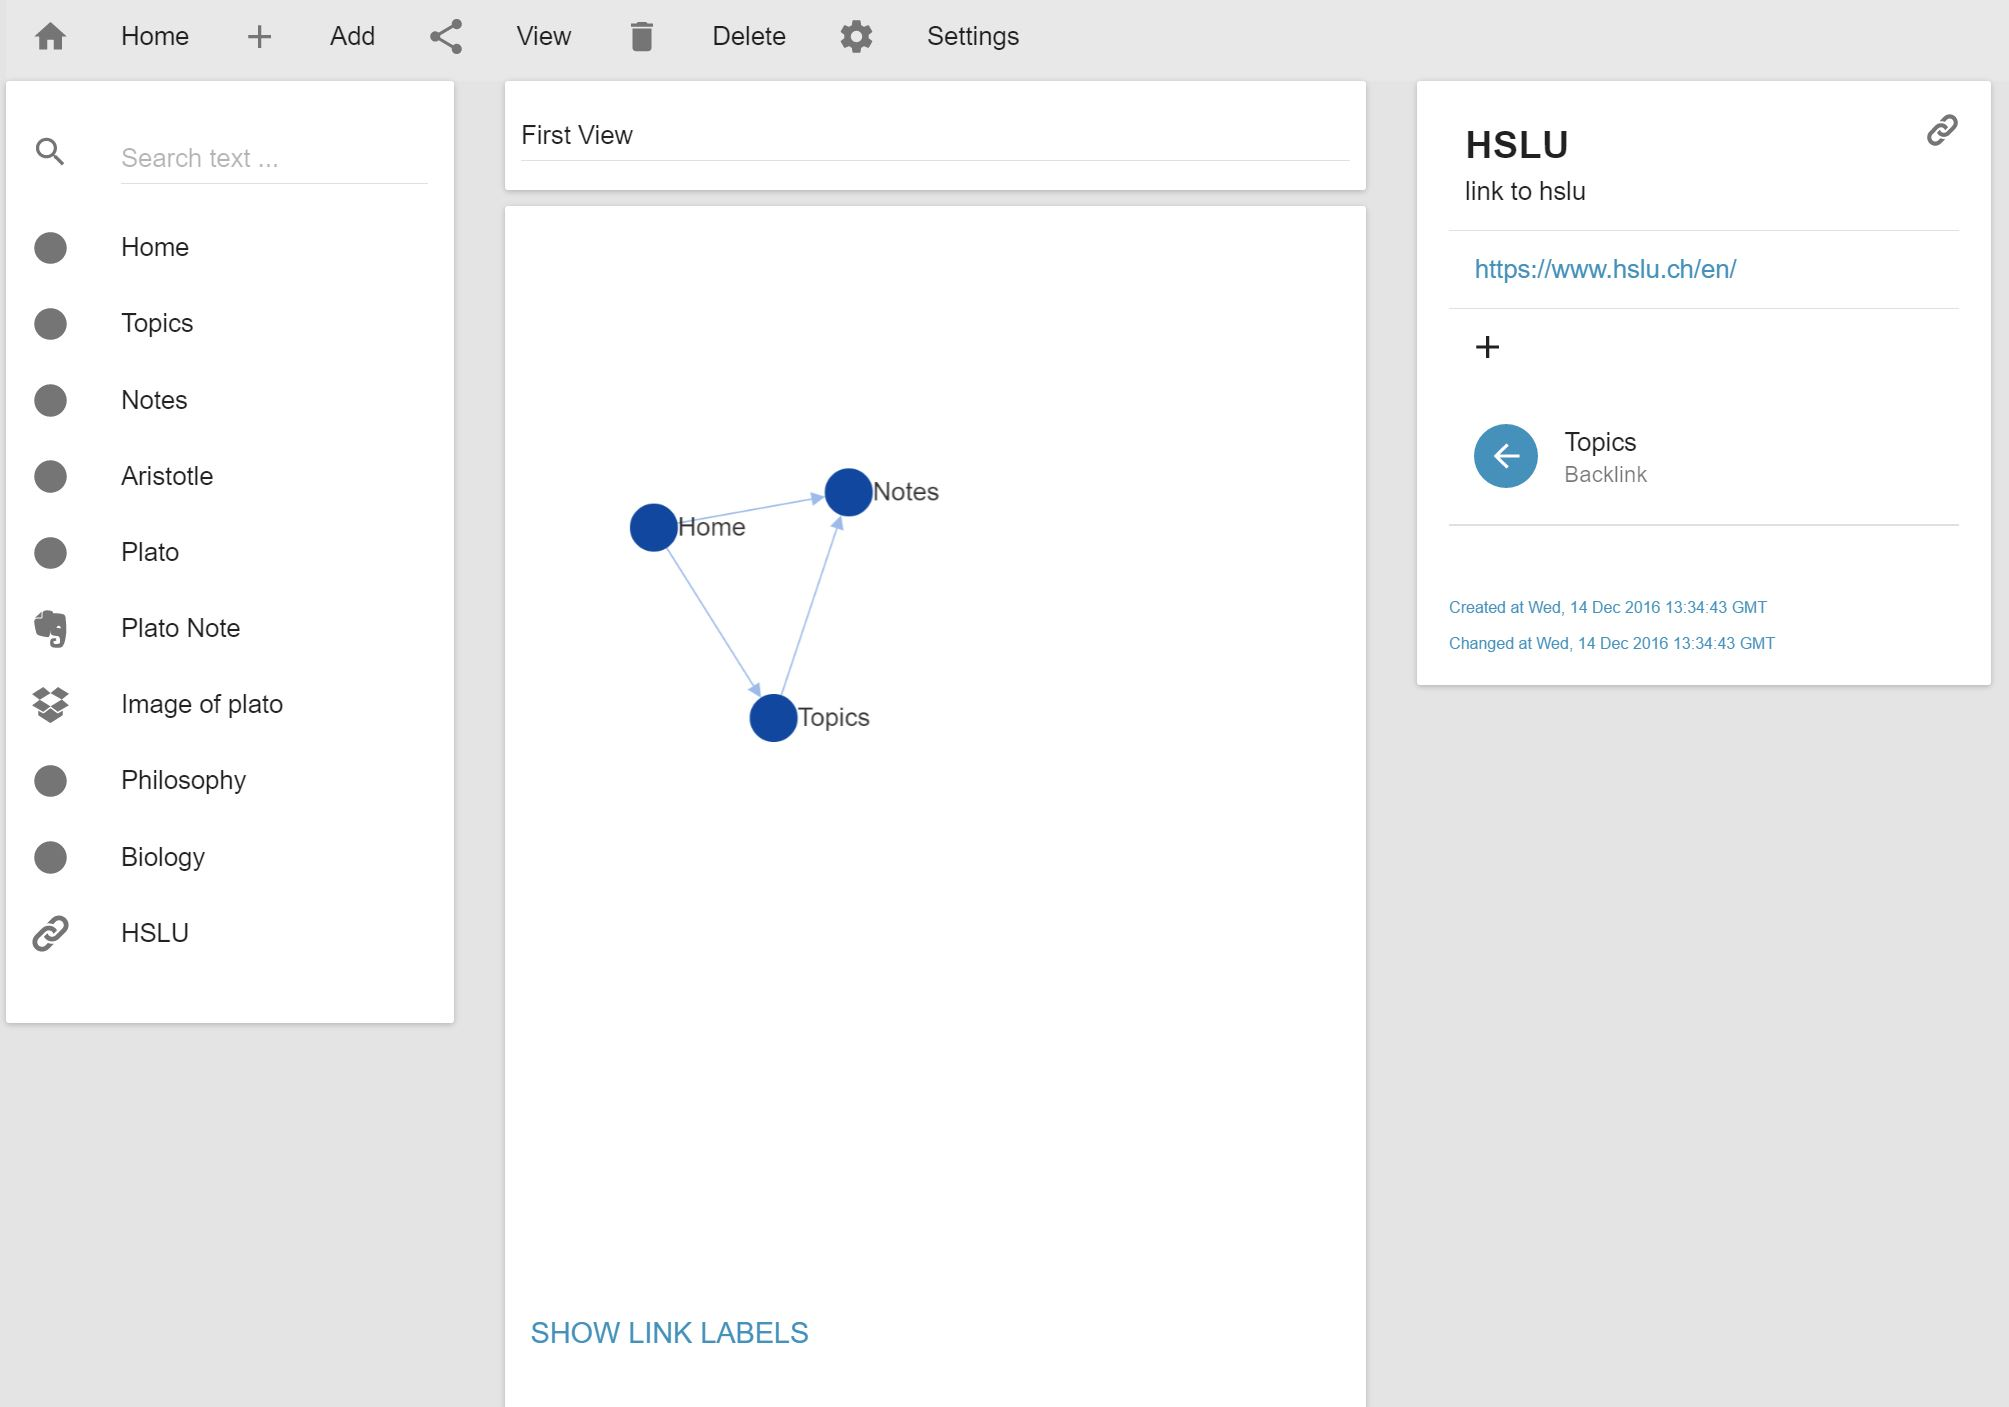
\includegraphics[width=1.3\textwidth]{Overview-Screen}}
\caption {Überblick Implementation}
\label{fig:overview-implementation}
\end{figure}

\section{Technologie} \label{sec:technologie}

Für die Umsetzung wurde aufgrund vieler Parallelen zum \gls{ikc-core} und diverser guten Erfahrungen auf ähnliche Technologien gesetzt. Das Grundgerüst ist daher nahezu identisch mit dem bisherigen. Dabei konnte bereits vorhandenes Wissen wiederverwendet und erweitert werden.

\subsection{Typescript}\label{typescript}

Typescript ist eine von Microsoft entwickelte statisch typisierte Erweiterung von Javascript. Durch die Kompilierung wird es zu üblichen Javascript. Typescript kann bereits während des Schreibens überprüft werden und die Entwicklungstools bieten dadurch viel Hilfestellung. Die Typen sind zwar optional, falls eingesetzt bringen sie aber einige hilfreiche Zusatzfunktionen. Beispielsweise lassen sich Klassen, Interfaces definieren. Dies ist vor allem bei der Entwicklung von grösseren Projekten hilfreich. \citep{typescriptlang}

Typescript wurde vor allem aufgrund der ein\-fach\-er\-en Struk\-tu\-rie\-rung von Projekten und der Typisierung eingesetzt. Zwar kann jegliche Ja\-va\-scri\-pt-Bibliothek eingebunden werden, aber ohne bereits vorhandene statische Typisierung in Form von \textit{Typings} bringt dies keine grossen Vorteile. Unglücklicherweise sind die Typisierungen noch nicht für alle Bibliotheken verfügbar und darum muss teilweise auf eine weniger elegante Integration ausgewichen werden.

\subsection{React}\label{react}

React ist eine Bibliothek für die Entwicklung von Benutzeroberflächen, entwickelt von Facebook. Der Fokus wird insbesondere auf die Interaktivität der Komponenten gelegt, deren Zustände ständig wechseln können. Bei Zustandsänderungen aktualisiert React automatisch alle notwendigen Komponenten. Die Komponentenbauweise bringt hohe Modularität und Wiederverwendbarkeit mit sich, untereinander sind die Komponenten entkoppelt. Einmal erstellte Komponenten können an beliebigen Stellen wiederverwendet werden, so zum Beispiel ein Suchfeld. Verwendet werden dies Komponenten immer in der \textit{XML}-Syntax. Grundsätzlich wird eine React-Komponente in verschiedene Teile zerlegt (\autoref{listing:react-component}): 

\begin{enumerate}
    \item \label{props} \textit{Props-Schnittstelle} - definiert, mit welchen Parameter eine Komponente benutzt werden muss. Optionale Parameter werden mit einem Fragezeichen (\texttt{\textbf{?}}) gekennzeichnet. Innerhalb der Komponente kann \texttt{this.props} auf die Eigenschaften zugreifen. Jedoch können keine Werte aktualisiert werden.
    \item \label{states} \textit{State-Schnittstelle} - spezifiziert den Zustand der Komponente. Diese kann sich abhängig von Ereignissen innerhalb der Komponente aktualisieren. Mit \texttt{this.state} kann ein Zugriff stattfinden.
    \item \textit{Implementierung} - jede Komponente implementiert die Schnittstelle \textit{React.Component$<>$}. Einzig die Methode \texttt{render} muss implementiert werden. Darin wird der darzustellende Inhalt aus \gls{HTML}-Elementen oder weiteren React-Komponenten zusammengestellt. 
    \item \textit{Verwendung} - nach der Implementierung kann jede Komponente von anderen React-Komponenten innerhalb deren \texttt{render} Methode verwendet werden.
\end{enumerate}

\begin{listing}[htbp]
\inputminted[
frame=lines,
framesep=2mm,
baselinestretch=1.2,
linenos,
breaklines=true
]{js}{sourcecode/common/react.ts}
\caption{Beispiel React Komponente}
\label{listing:react-component}
\end{listing}

Jede React-Komponente durchläuft grundlegende Zustände. An diesen kann mit sogenannten \textit{Lifecycle}-Methoden in den jeweiligen Prozess eingegriffen werden. Bei der Implementierung der Visualisierung wurden hauptsächlich folgenden Methoden eingesetzt.
%Zusätzlich durchläuft jede React-Komponente drei grundlegende Zustände, in welchen mit verschiedenen speziellen Methode darauf reagiert werden kann:

\begin{itemize}
   \item \textit{Mounting} - hier werden verschiedene Methoden abgearbeitet, bis eine Komponente erstellt und zu einem \gls{HTML}-Element konvertiert wird.
   \begin{enumerate}
     \item \texttt{constructor}
     \item \texttt{componentWillMount}
     \item \texttt{render}
     \item \texttt{componentDidMount}
   \end{enumerate}
   \item \textit{Updating} - ein Update kann entweder durch eine Aktualisierung des \textit{State} oder der \textit{Props} erfolgen.
   \begin{enumerate}
     \item \texttt{componentWillReceiveProps}
     \item \texttt{shouldComponentUpdate}
     \item \texttt{componentWillUpdate}
     \item \texttt{render}
     \item \texttt{componentDidUpdate}
   \end{enumerate}
   \item \textit{Unmounting} - dieser Schritt wird ausgeführt, bevor die Komponente entfernt wird.
   \begin{enumerate}
     \item \texttt{componentWillUnmount}
   \end{enumerate}
\end{itemize}

Ein weiterer, besonderer Punkt von React ist der uni\-di\-rek\-tio\-nale Datenfluss. Dieser wird nachfolgend im \autoref{unidirectional} behandelt. \citep{reactjs, reactjs-blog}

\subsection[Datenfluss]{Unidirektionaler Datenfluss}\label{unidirectional}
Die Verwendung von unidirektionalen Datenflüssen erleichtert die Verwendung von React-Komponenten, welche auch in dem, von Facebook präsentierten, Architektur-Muster \textit{Flux} enthalten sind. Auf eine strikte Verwendung von \textit{Flux} wurde verzichtet, jedoch wurden trotzdem unidirektionale Datenflüsse eingesetzt. Wie diese genau funktionieren, wird anhand des Beispiels in \autoref{fig:unidirectional} genauer aufgezeigt: 
   \begin{enumerate}
     \item Die \textit{GraphScreen}-Komponente verwendet die \textit{Graph}-Komponente in ihrer \texttt{render}-Methode in Form von (\texttt{<Graph ... />}). 
     \item Sobald den \textit{Graph}-Komponente erstellt ist, wird der Zustand anhand der übergebenen Parameter initialisiert.
     \item Angestossen von \gls{Event}s aus dem \textit{cytoscape}-Framework werden \gls{Callback}-Methoden aufgerufen, um Information an die \textit{GraphScreen}-Komponente zu senden. Die entsprechenden Methoden werden als Parameter an die \textit{Graph}-Komponente übergeben, beispielsweise \texttt{this.prop.handleNewLink(...)}
     \item Innerhalb den von der \textit{Graph}-Komponente aufgerufenen Methoden in der \textit{GraphScreen}-Komponente wird nun der Zustand der \textit{GraphScreen}-Komponente aktualisiert. Dies geschieht mit der Methode \texttt{this.setState({...})}, welche von dem React-Framework zur Verfügung gestellt wird. Hier werden die Änderungen weitergegeben. Diese werden im Hintergrund ausgeführt.
     \item Sobald der Zustand angepasst wurde, wird die \texttt{render}-Methode neu ausgeführt. Dadurch werden die Aktualisierungen der \textit{Graph}-Komponente per Parameter (\textit{Props}) weitergegeben.
     \item Durch die Aktualisierung der Parameter wird nun auch die \texttt{render} Methode der \textit{Graph}-Komponente neu ausgeführt und der Zustand aktualisiert. 
   \end{enumerate}

\begin{figure}[htbp]
\centerline{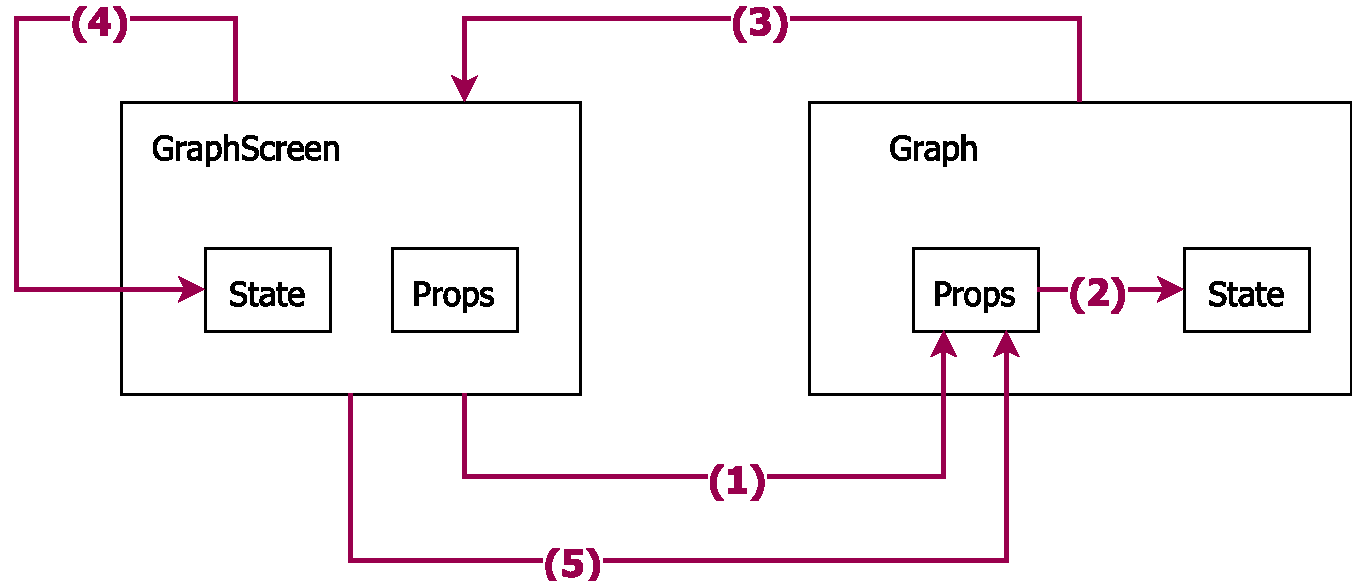
\includegraphics[width=1\textwidth]{unidirectional}}
\caption {Unidirektionaler Datenfluss}
\label{fig:unidirectional}
\end{figure}


\subsection{Material Design}

Die React Erweiterung \textit{Material UI} ist zuständig für das Erscheinungsbild der Visualisierung, wie auch schon beim \textit{ikc-core}. Dafür gibt es diverse vorgefertigte Komponenten, welche praktisch ohne Zusatzaufwand verwendet werden können. Googles Material Design kombiniert klassische Design Prinzipien mit Innovation auf Technik und Wissenschaft. \citep{react-material-ui, google-material-ui}

\subsection{Webpack}

Mit der Verwendung von zahlreichen Erweiterungen und \hyperref[typescript]{\textit{Typescript}} als primäre Programmiersprache ergeben sich diverse Abhängigkeiten und auch eine Kompilierung ist notwendig. Für die Sammlung der Abhängigkeiten und die Übersetzung in Javascript wird Webpack eingesetzt. Das Resultat ist beispielweise eine Javascript-Datei, welche alle Abhängigkeiten im richtigen Format enthält. Darum ist vom Webserver nur eine Datei zu laden, so verkürzt die Ladezeit zusätzlich. \citep{webpack}

\section[Interkation]{Interaktion mit bestehenden Komponenten}\label{interaktion}

Innerhalb der Visualisierung werden verschiedene bestehende Komponenten aus dem \gls{ikc-core} genutzt. Diese implementieren die beschriebenen Schnittstellen (\autoref{schnittstellen}) und werden an den \textit{GraphScreen} üb\-er\-ge\-ben. Die Implementationen gelten als Voraussetzung für die Verwendung der Visualisierung.

\subsubsection{GraphDialogFactory/GraphSearchFieldFactory}
Mit Hilfe dieser beiden Klassen kann die Visualisierung auf \hyperref[react]{\textit{React}}-Komponenten zugreifen, welche im \gls{ikc-core} implementiert sind. Diese sind in erster Linie Dialoge oder Suchfelder. Im folgenden Ablaufdiagramm (\autoref{fig:interaction-dialog} und \autoref{listing:interaction-factory}) ist die Funktionsweise am Beispiel des \textit{NewNodeDialog}s detailliert ersichtlich. Das Prinzip gilt ebenfalls für die Dialoge \textit{NewNodeToConnect}, \textit{NodeSearchToConnect} und die beiden Suchfelder \textit{NodeSearchField} und \textit{LinkSearchField}:

\begin{enumerate}
    \item Die Komponente \textit{GraphVisualisation} erstellt ein Objekt der Klasse \textit{GraphDialogFactory}. Sie implementiert die Schnittstelle \hyperref[DialogFactory]{\textit{DialogFactory}} aus der Visualisierung.
    \item Bei der Verwendung der Visualisierung (\textit{GraphScreen}) wird unter anderem das \textit{GraphDialogFactory}-Objekt an die Visualisierung übergeben. Dabei ändert das Objekt den Typ von \textit{GraphDialogFactory} zu \hyperref[DialogFactory]{\textit{DialogFactory}}. Da ersteres der Visualisierung unbekannt ist, kann so eine beidseitige Kopplung verhindert werden. Alle Objekte, welche übergeben werden, sind in der Schnittstelle \hyperref[GraphScreenProps]{\textit{GraphScreenProps}} zusammengefasst. Diese wird innerhalb des \hyperref[react]{\textit{React}}-Frameworks implementiert.
    \item Wenn nun die Visualisierung einen \textit{NewNode}-Dialog benötigt, wird dieser von der \textit{GraphDialogFactory} bezogen. Diese wird von dem \hyperref[GraphScreenProps]{\textit{GraphScreenProps}} zur Verfügung gestellt. Dazu wird die Methode \texttt{getNewNodeDialog} aufgerufen, welcher die benötigten Informationen für die Erstellung des Dialogs mitgegeben werden.
    \item Nachdem der Dialog geschlossen wurde, werden die entsprechenden \gls{Callback}-Methoden ausgeführt. Diese stehen dem Dialog durch das \textit{DialogNewNodeProps}-Objekt zu Verfügung, welches zuvor von der \textit{GraphDialogFactory} anhand der Informationen der Visualisierung entsprechend bestückt wurde. Somit wird die Visualisierung über das Resultat des Dialogs informiert und kann die Informationen entsprechend weiterverarbeiten. 
\end{enumerate}

\begin{figure}[htbp]
\centerline{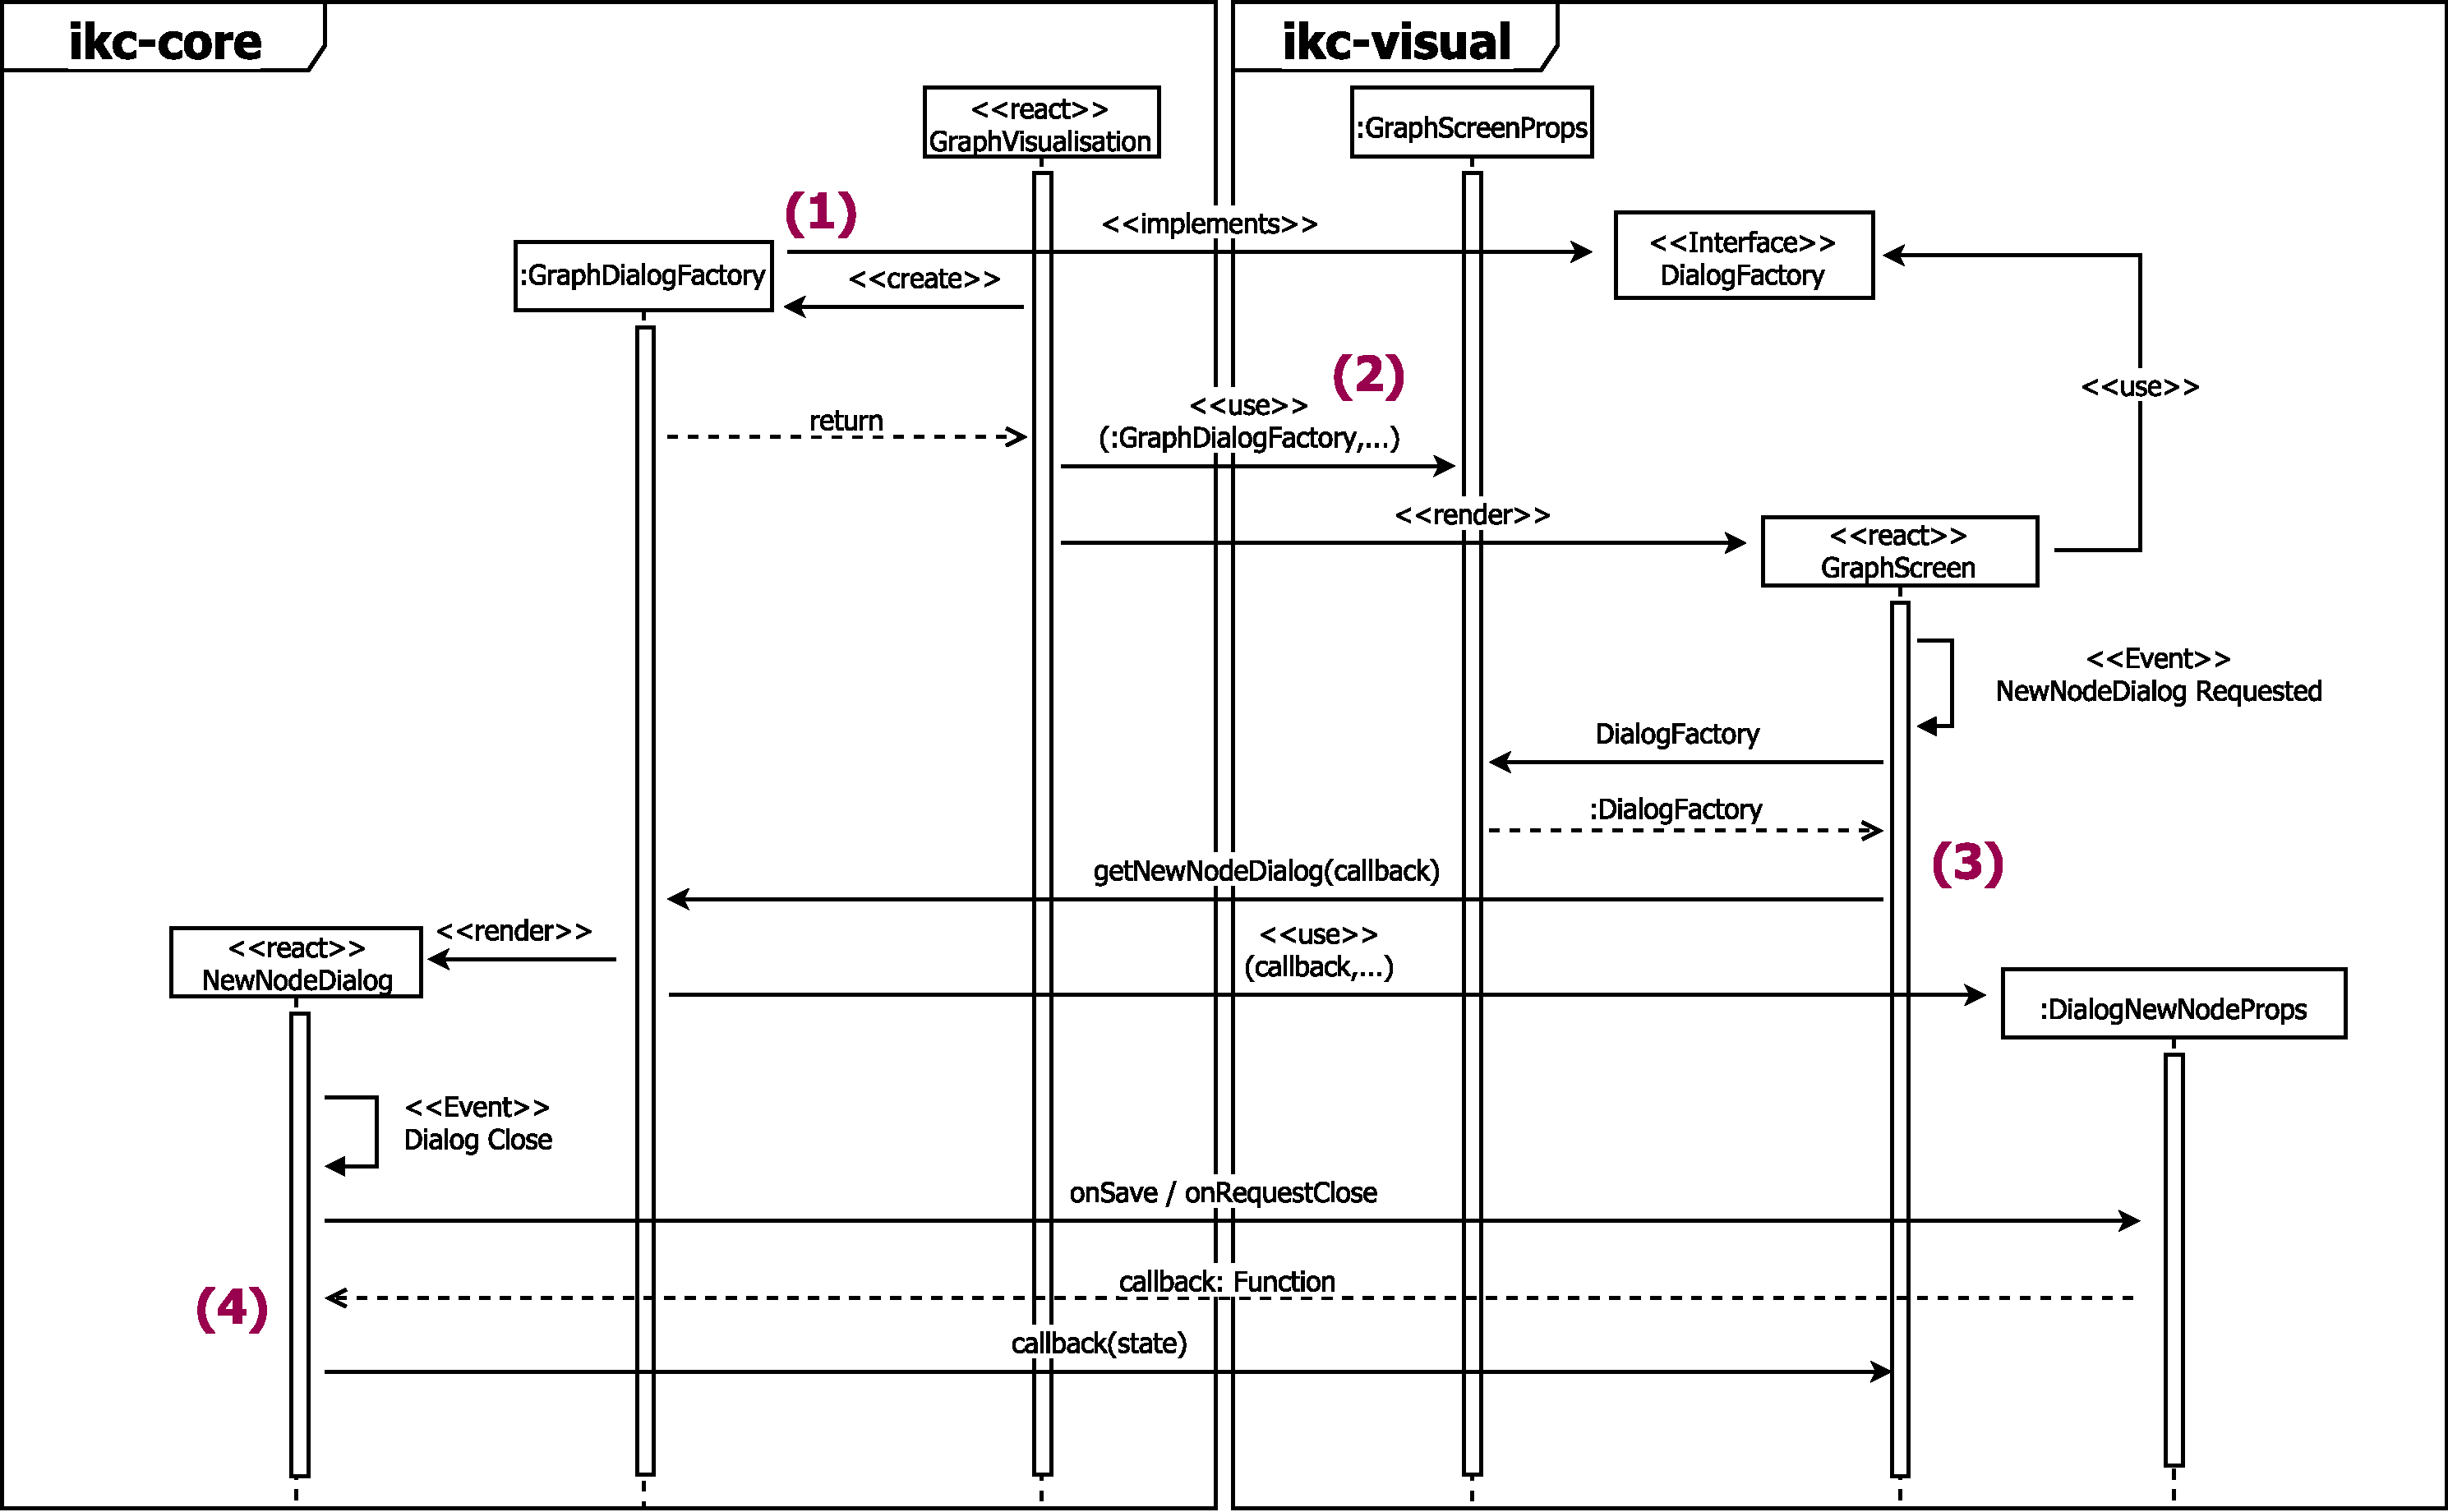
\includegraphics[width=1.3\textwidth]{ExternalComponentDialog}}
\caption{Interaktion mit den Factories}
\label{fig:interaction-dialog}
\end{figure}

\begin{listing}[htbp]
\inputminted[
frame=lines,
framesep=2mm,
baselinestretch=1.2,
linenos,
breaklines=true
]{js}{sourcecode/common/InteractionFactory.ts}
\caption{Beispiel Interaktion Factory}
\label{listing:interaction-factory}
\end{listing}

\subsubsection{Weitere Implementationen}
Mit Hilfe der Implantation der Schnittstellen \hyperref[NodeInformationProvider]{\textit{NodeInformationProvider}},  \hyperref[OperationService]\textit{OperationService},  \hyperref[IdentityService]{\textit{IdentityService}} können der Visualisierung konkrete Implementationen zu Verfügung gestellt werden (\autoref{fig:interaction-nodeinformationprovider}, \autoref{fig:interaction-identityservice}, \autoref{fig:interaction-operationservice} und \autoref{listing:interaction-components}):
\begin{enumerate}
    \item Das entsprechende Objekt der Implementierung wird erstellt.
    \item Bei der Erstellung der Visualisierung wird das Objekt übergeben.
    \item Über \hyperref[GraphScreenProps]{\textit{GraphScreenProps}} kann die Visualisierung auf das entsprechende Objekt zugreifen und mit den Methoden die benötigten Informationen abrufen.
\end{enumerate}

\begin{figure}[htbp]
\centerline{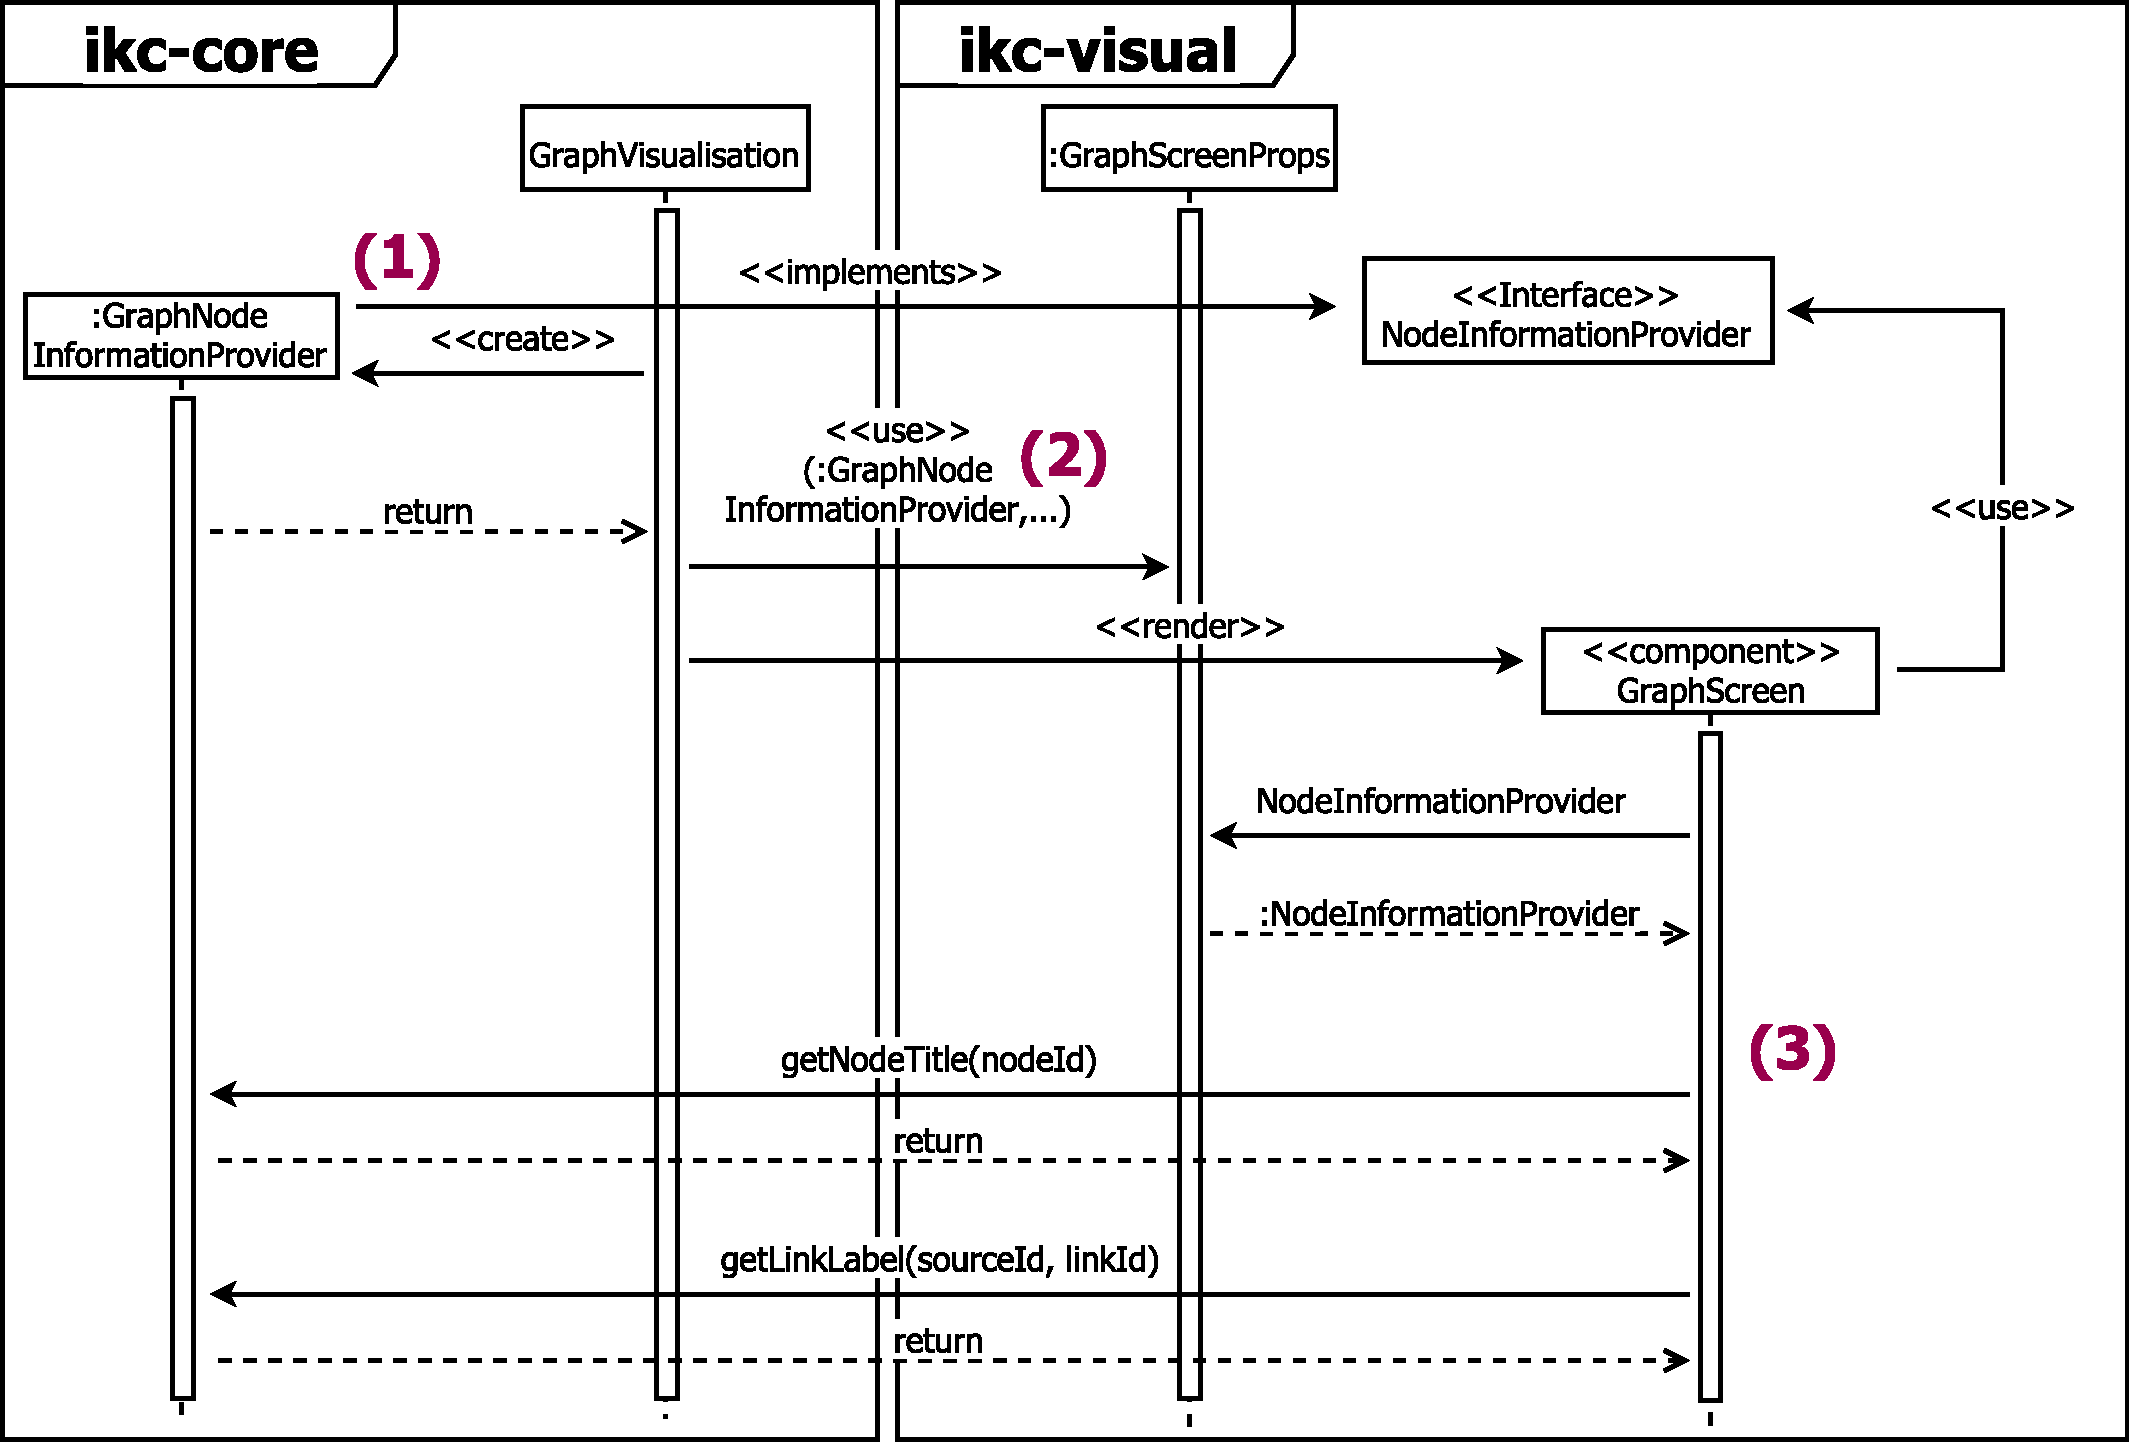
\includegraphics[width=1.3\textwidth]{ExternalComponentInformationProvider}}
\caption{Interaktion mit dem NodeInformationProvider}
\label{fig:interaction-nodeinformationprovider}
\end{figure}


\begin{figure}[htbp]
\centerline{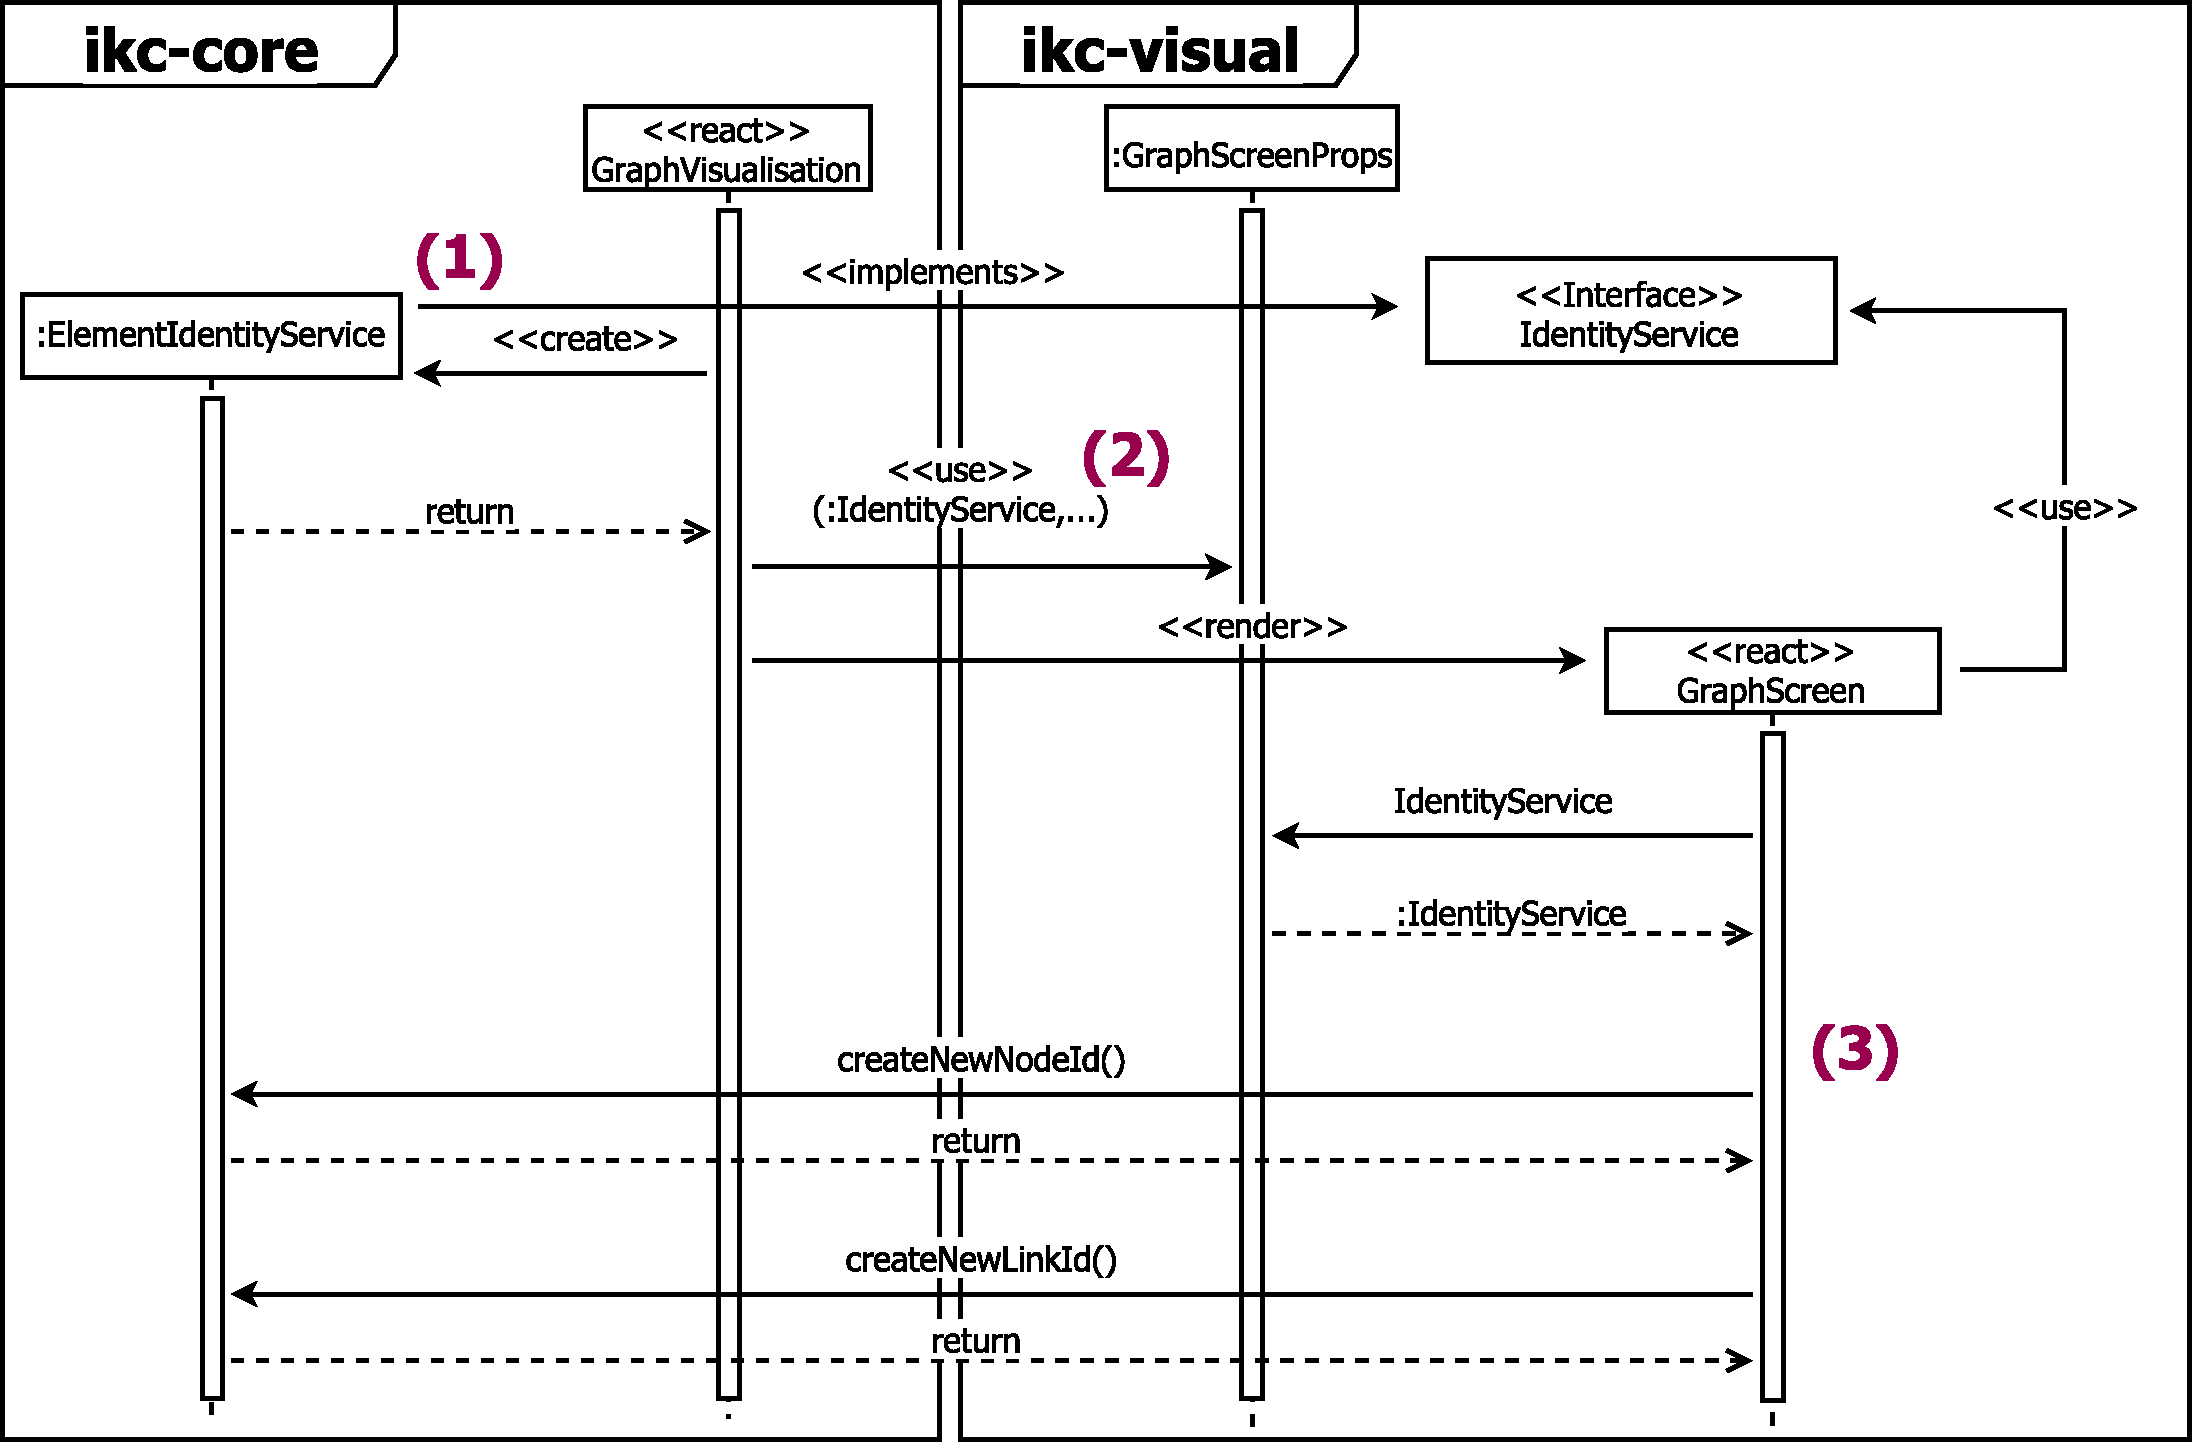
\includegraphics[width=1.3\textwidth]{ExternalComponentIdentityService}}
\caption{Interaktion mit dem IdentityService}
\label{fig:interaction-identityservice}
\end{figure}


\begin{figure}[htbp]
\centerline{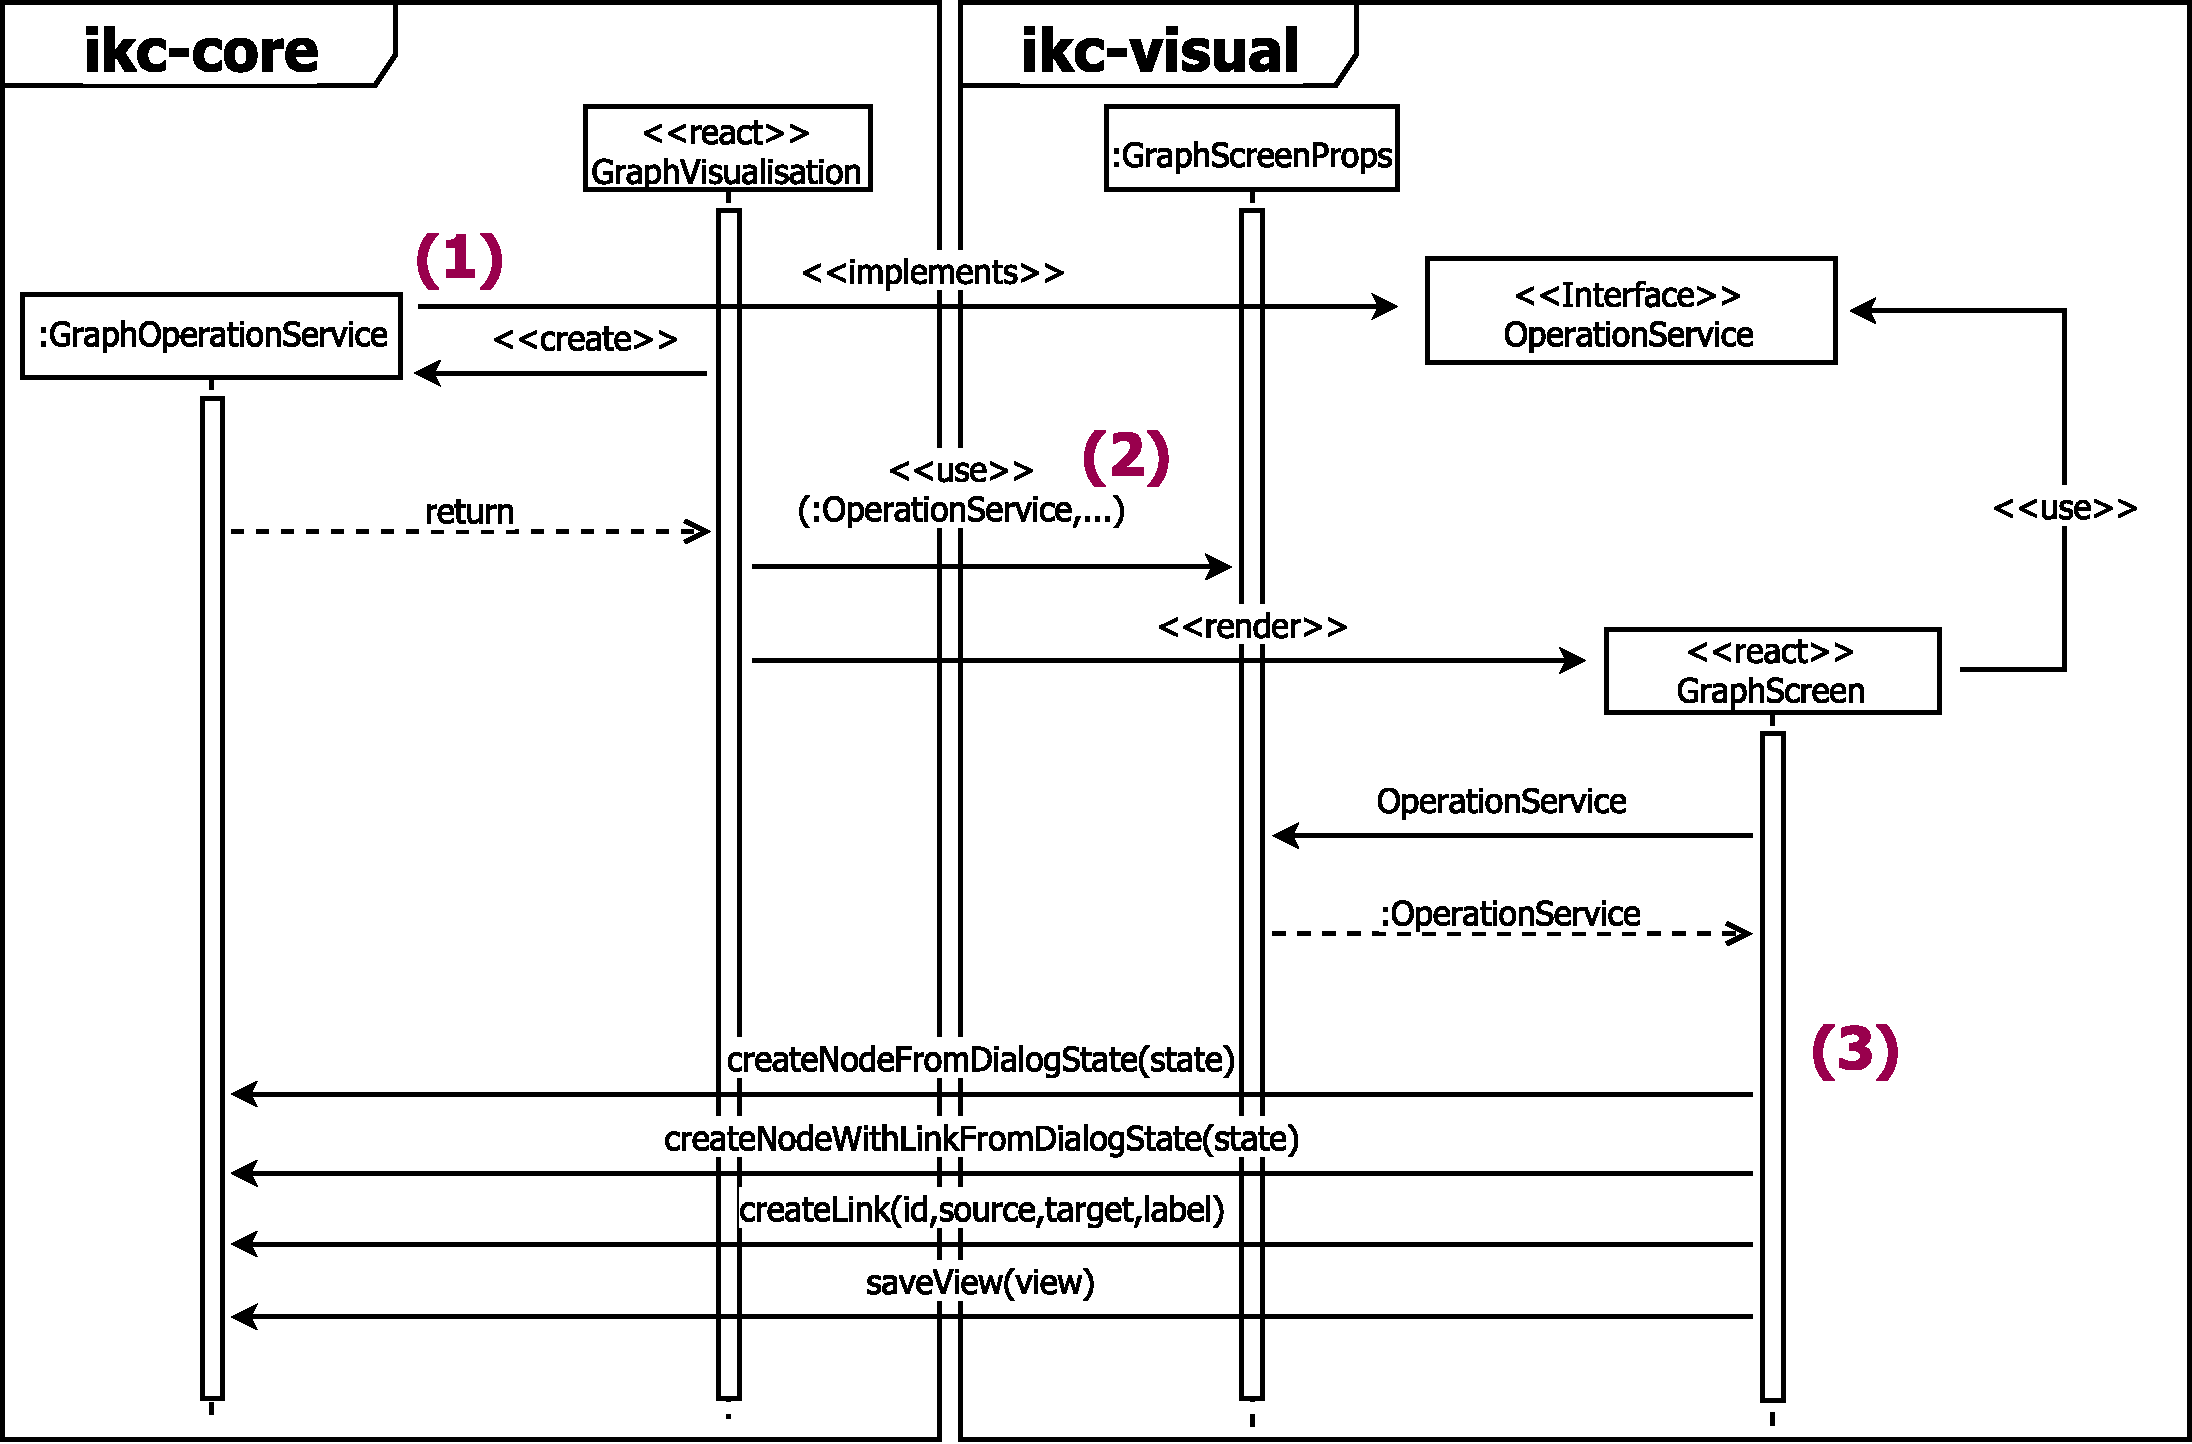
\includegraphics[width=1.3\textwidth]{ExternalComponentOperationService}}
\caption{Interaktion mit dem OperationService}
\label{fig:interaction-operationservice}
\end{figure}

\begin{listing}[htbp]
\inputminted[
frame=lines,
framesep=2mm,
baselinestretch=1.2,
linenos,
breaklines=true
]{js}{sourcecode/common/InteractionComponents.ts}
\caption{Beispiel: Interaktion weiterer Komponenten}
\label{listing:interaction-components}
\end{listing}

\section{Drag'n'Drop}
\label{dnd}
Die \gls{Drag'n'Drop}-Funktionalität bietet sowohl auf dem mobilen als auch auf dem Desktop-Gerät die Möglichkeit, Benutzerinteraktion intuitiv und einfach zu gestalten. Wie im \autoref{subsec:aktionen} bereits definiert, sind dies \textit{Add Node}, \textit{New Link}, \textit{Link To Existing Node} und \textit{Update Position}. Dies kann sowohl innerhalb der Visualisierung oder auch von einer externen Komponente aus geschehen. In diesem Abschnitt werden die grundsätzlichen Abläufe erläutert, welche es ermöglichen einen \gls{Node} von einer externen Komponente in die Visualisierung zu ziehen. Wie die Aktionen innerhalb der Visualisierung funktionieren, wird im \autoref{subsec:graph-manipulation} erläutert.

Grundsätzlich wird der Vorgang des \gls{Drag'n'Drop}[s] in vier Phasen unterteilt:

\begin{itemize}
    \item \textit{Registration} - Alle Elemente, auf welche ein Drag (Nodes) oder ein Drop (Visualisierung) möglich sein soll, müssen registriert werden. 
    \item \textit{Drag} - Ein Drag wird mit einem Klick oder Tap auf einem Element gestartet.
    \item \textit{Move} - Das Element wird auf dem Monitor bewegt.
    \item \textit{Drop} - Das Element wird auf der Visualisierung losgelassen. Wenn dies an einer freien Stelle geschieht, wird der \gls{Node} an dieser Stelle hinzugefügt (4.a). Geschieht dies jedoch über einem bestehenden \gls{Node}, wird ein neuer \gls{Link} erstellt und der neue \gls{Node} im Umkreis des bestehenden positioniert (4.b).
\end{itemize}


\begin{figure}[htbp]
\centerline{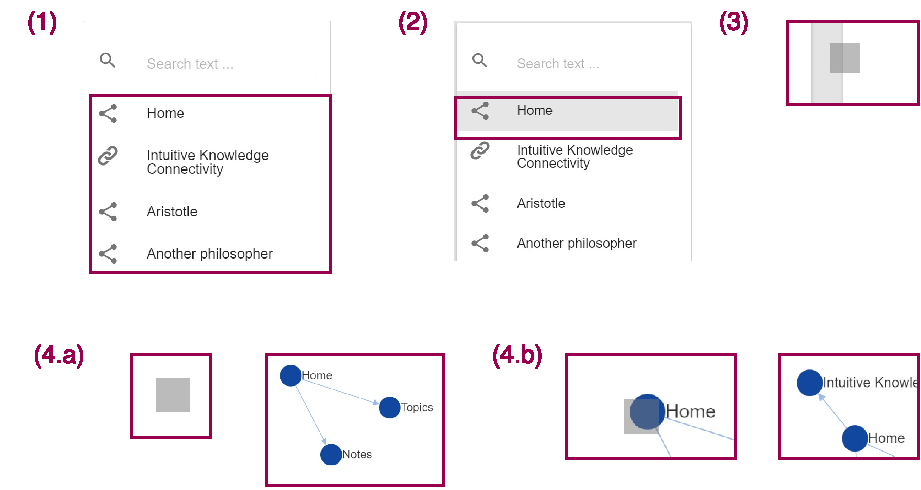
\includegraphics[width=1.3\textwidth]{DragNDropScreen}}
\caption{Übersicht \gls{Drag'n'Drop}}
\label{fig:dnd-screen}
\end{figure}

Damit diese Phasen korrekt ausgeführt werden können, ist es wichtig zu wissen, welcher \gls{Node} an der Aktion beteiligt ist. Weiter müssen verschiedene \gls{Event}s abgefangen und verarbeitet werden. Um dies möglichst simpel und effizient zu implementieren, wird dies in eine externe \gls{Javascript}-Datei ausgelagert und somit vom Rest entkoppelt (\autoref{listing:dnd-handling}). Dieses bietet zwei zwingende und zwei optionale Methoden:
\begin{itemize}
    \item \textit{registerDragZone} - Mit der Registration wird das \gls{Drag'n'Drop} auf dem entsprechenden \gls{HTML}-Element aktiviert. Dazu muss das entsprechende \gls{HTML}-Objekt als auch die entsprechende Node-ID übergeben werden.
    \item \textit{registerDropZone} - Ebenfalls muss die Visualisierung als Drop-Zone registriert werden. Dadurch kann bei einem Drop über ihr die \gls{Callback}-Methode \textit{onDrop} ausgeführt werden, welche übergeben werden muss. 
    \item \textit{registerCallbackForStart} - Hiermit wird jedem Element ermöglicht, bei einem Start eines \gls{Drag'n'Drop} informiert zu werden. 
    \item \textit{registerCallbackForEnd} - Dadurch ist es möglich benachrichtigt zu werden, sobald der \gls{Drag'n'Drop}-Vorgang beendet ist.
\end{itemize}

\begin{listing}[htbp]
\inputminted[
frame=lines,
framesep=2mm,
baselinestretch=1.2,
linenos,
breaklines=true
]{js}{sourcecode/common/MobileDrop.js}
\caption{Drag'n'Drop Handhabung}
\label{listing:dnd-handling}
\end{listing}

Wie diese Phasen im Detail abgehandelt wird, ist in Ablaufdiagramm (\autoref{fig:dnd-sequence}) ersichtlich. Sie sind ebenfalls in die vier Phasen des \gls{Drag'n'Drop} unterteilt.

\begin{figure}[htbp]
\centerline{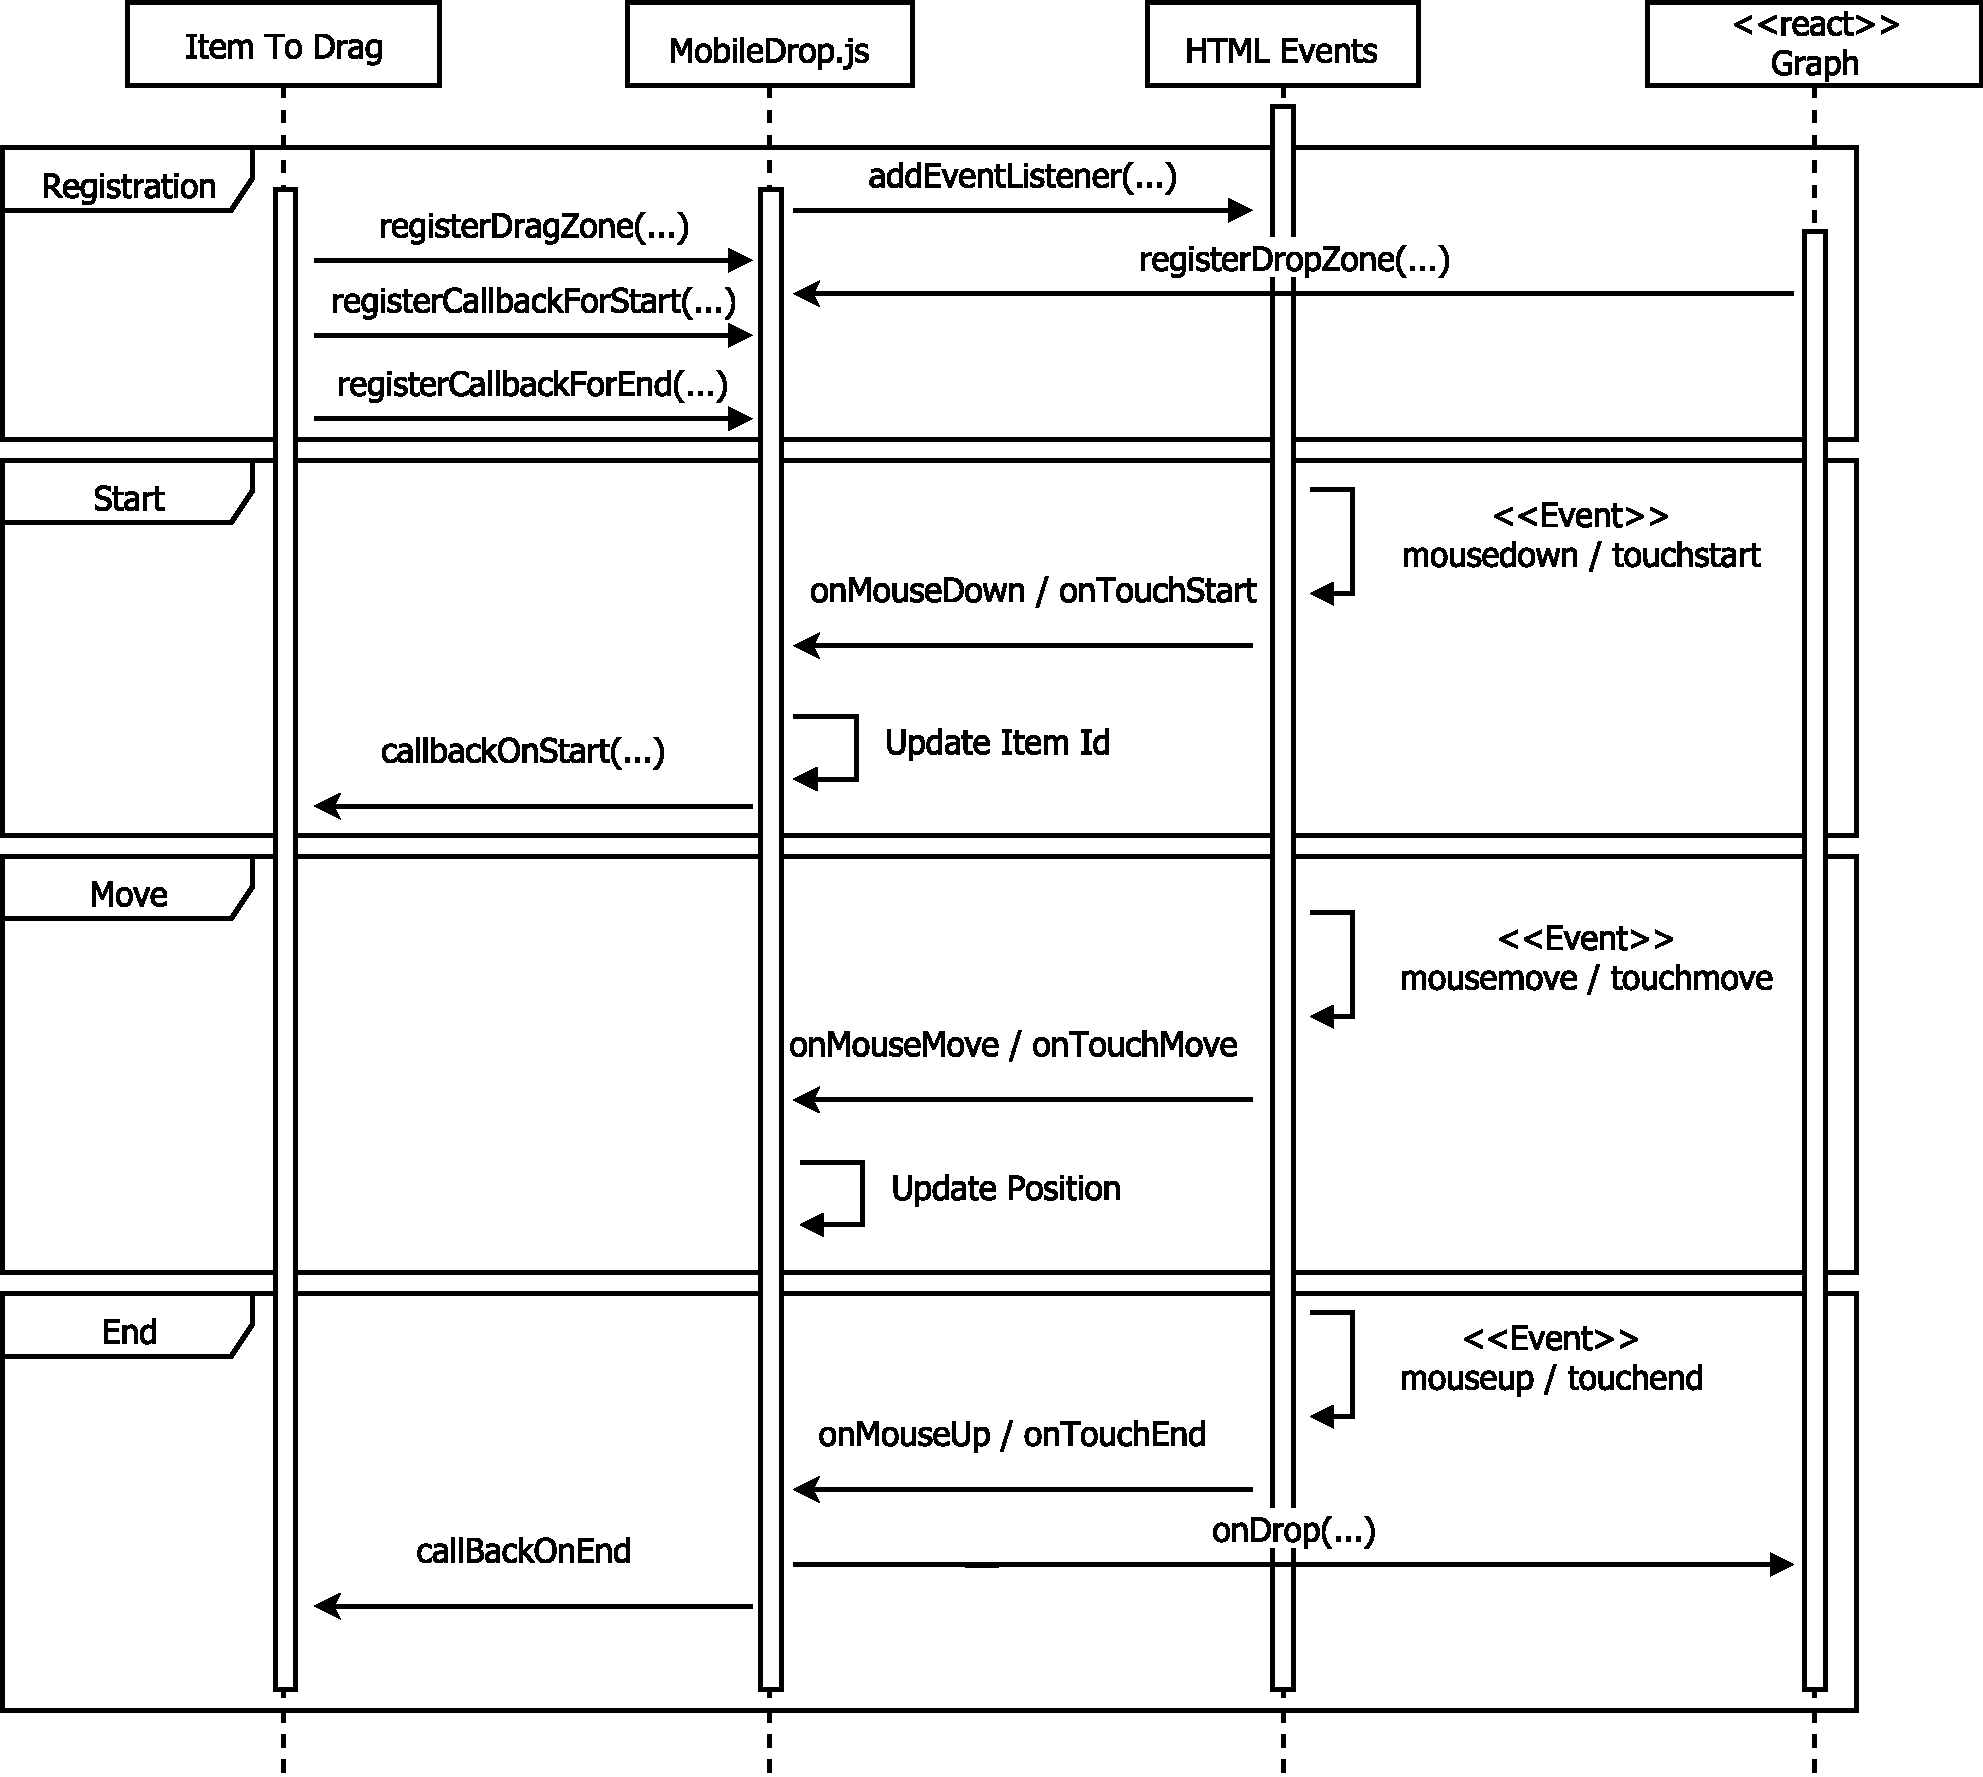
\includegraphics[width=1.2\textwidth]{DragAndDrop}}
\caption{Ablauf \gls{Drag'n'Drop}}
\label{fig:dnd-sequence}
\end{figure}

\section{Visualisierung}\label{visual}
Die Funktionalitäten der Visualisierung werden hauptsächlich durch vier \hyperref[react]{\textit{React}}-Komponenten abgedeckt: \textit{GraphScreen} fungiert dabei als zentrale Stelle und initialisiert alle anderen Komponenten. Insbesondere wird das entsprechende \hyperref[view]{\textit{View}}-Objekt, \textit{viewToLoad} analysiert, die darzustellenden \gls{Node}[s] und \gls{Link}[s] extrahiert und der \textit{Graph}-Komp\-on\-en\-te übergeben.

Sobald innerhalb der Visualisierung ein \gls{Event} aufgrund einer Benutzerinterkation ausgelöst wird, werden die entsprechenden \gls{Callback}-Methoden des \textit{GraphScreen} aufgerufen. Darüber werden die entsprechenden Schritte ausgeführt, welche wiederum zu Aktualisierungen in den einzelnen Komponenten führen (\autoref{fig:component-visualisation}). Jegliche Kommunikation zwischen den Komponenten wird nach dem Prinzip des unidirektionalen Datenflusses (\autoref{unidirectional}) realisiert.

Zum Beispiel soll ein \gls{Link} dargestellt werden. Dazu wird im \textit{GraphScreen} beim entsprechenden \hyperref[GraphLinkElement]{Link} die Eigenschaft \textit{visible} auf \texttt{VISI\-BILI\-TY.VISI\-BLE} gesetzt. Durch die Aktualisierung des Zustands werden nun die \gls{Node}[s] und \gls{Link}[s], welche der \textit{Graph}-Komponente übergeben werden, aktualisiert. Darin enthalten ist nun auch der neu darzustellende Link.

\begin{figure}[htbp]
\centerline{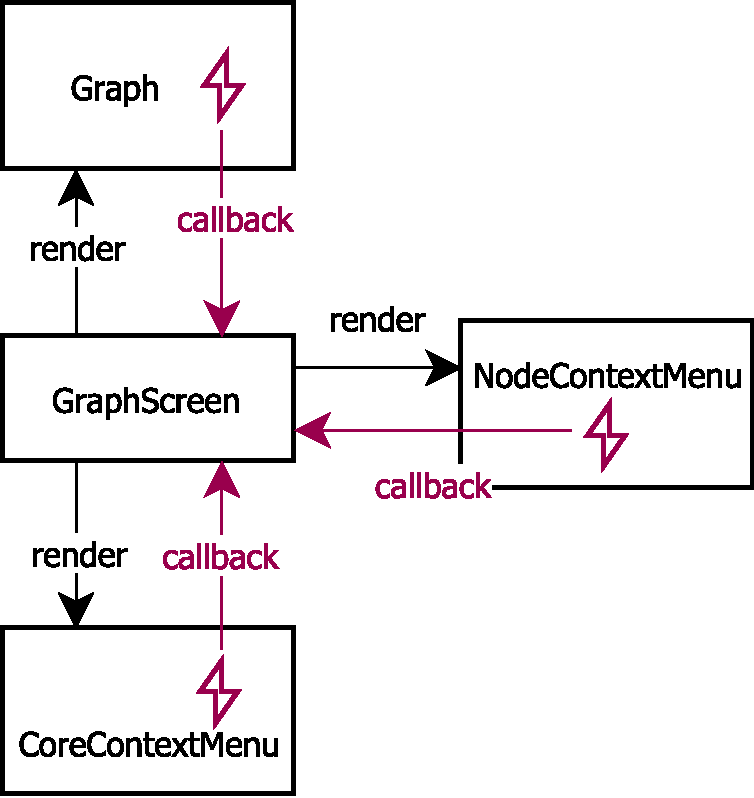
\includegraphics[width=0.5\textwidth]{VisualisationComponents}}
\caption{Komponenten der Visualisierung}
\label{fig:component-visualisation}
\end{figure}


\subsection{Manipulation des \gls{Netzwerk}[s]}
\label{subsec:graph-manipulation}

Die Manipulationen innerhalb des \gls{Netzwerk}[s] haben ihren Ursprung immer im \textit{cytoscape}-Framework. Hier werden verschiedene \gls{Event}s registriert, um entsprechend reagieren zu können. Dies geschieht auf verschiedenen Ebenen der Visualisierung:
\begin{enumerate}
    \item Auf der ganzen Visualisierung, zum Beispiel \textit{Rechtsklick} an einer freien Stelle.
    \item Auf mehreren \gls{Node}[s] der Visualisierung, zum Beispiel \textit{durch Auswahl}.
    \item Auf mehreren \gls{Link}[s] der Visualisierung, zum Beispiel durch \textit{Auswahl}.
    \item Auf einem spezifischen Element der Visualisierung, zum Beispiel \textit{Loslassen} eines \gls{Node}[s].
\end{enumerate}


\begin{listing}[htbp]
\inputminted[
frame=lines,
framesep=2mm,
baselinestretch=1.2,
linenos,
breaklines=true
]{js}{sourcecode/common/cytoscape-event.ts}
\caption{Cytoscape Event Beispiel}
\label{listing:cytoscape-event}
\end{listing}

\subsubsection{Update Position/New Link (Drag'n'Drop)}
Wenn die Aktion \textit{Update Position} und \textit{New Link} per \gls{Drag'n'Drop} ausgeführt werden, startet ein teilweise ähnlicher Ablauf (\autoref{fig:sequence-movenode}):
\begin{enumerate}
    \item Der erste Schritt ist Teil des allgemeinen Ablaufs der Visualisierung. Darin wird die \textit{Graph}-Komponente erstellt. Falls eine Aktion auf einem \gls{Node} ausgeführt wird, wird der \gls{Event} \textit{grab} registriert.
    \item Bei der Auswahl und Bewegung eines \gls{Node}[s], wird nun der \gls{Event} \textit{free} temporär registriert, welcher ausgeführt wird sobald der \gls{Node} losgelassen wird.
    \item Sobald der \gls{Node} losgelassen wird, wird überprüft, ob an dieser Stelle in der Visualisierung ein anderer \gls{Node} positioniert ist. Ist dies der Fall, wird ein neuer \gls{Link} zwischen den zwei \gls{Node}[s] erstellt und dazu folgende Schritte ausgeführt:  
        \begin{itemize}
            \item Die \textit{GraphScreen}-Komponente wird mittels einer \textit{Callback}-Meth\-ode informiert.
            \item Innerhalb der \textit{GraphScreen}-Komponente wird der neue \gls{Link} erstellt und die Datenbasis durch den \hyperref[OperationService]{\textit{OperationService}} informiert.
            \item Nun wird der Zustand der \textit{GraphScreen}-Komponente aktualisiert, die \texttt{render}-Methode ausgeführt und die Aktualisierungen an die \textit{Graph}-Komponente weitergegeben. Zum Schluss werden die Änderungen angezeigt.    
        \end{itemize}
    Wenn dies jedoch nicht zutrifft, werden folgende Schritte ausgeführt. So kann die neue Position des \gls{Node}[s] gespeichert werden: 
        \begin{itemize}
            \item Durch die entsprechende \textit{Callback}-Methode wird die \textit{GraphScreen}-Komponente informiert.
            \item Die Position wird innerhalb der \textit{GraphScreen}-Komponente aktualisiert und die Datenbasis durch den \hyperref[OperationService]{\textit{OperationService}} informiert.
            \item Ebenfalls wird der Zustand der \textit{GraphScreen}-Komponente aktualisiert, die \texttt{render} Methode ausgeführt und die Aktualisierungen an die \textit{Graph}-Komponente weitergegeben. Wiederum werden zum Schluss die Änderungen sichtbar.
        \end{itemize}
\end{enumerate}

\begin{figure}[htbp]
\centerline{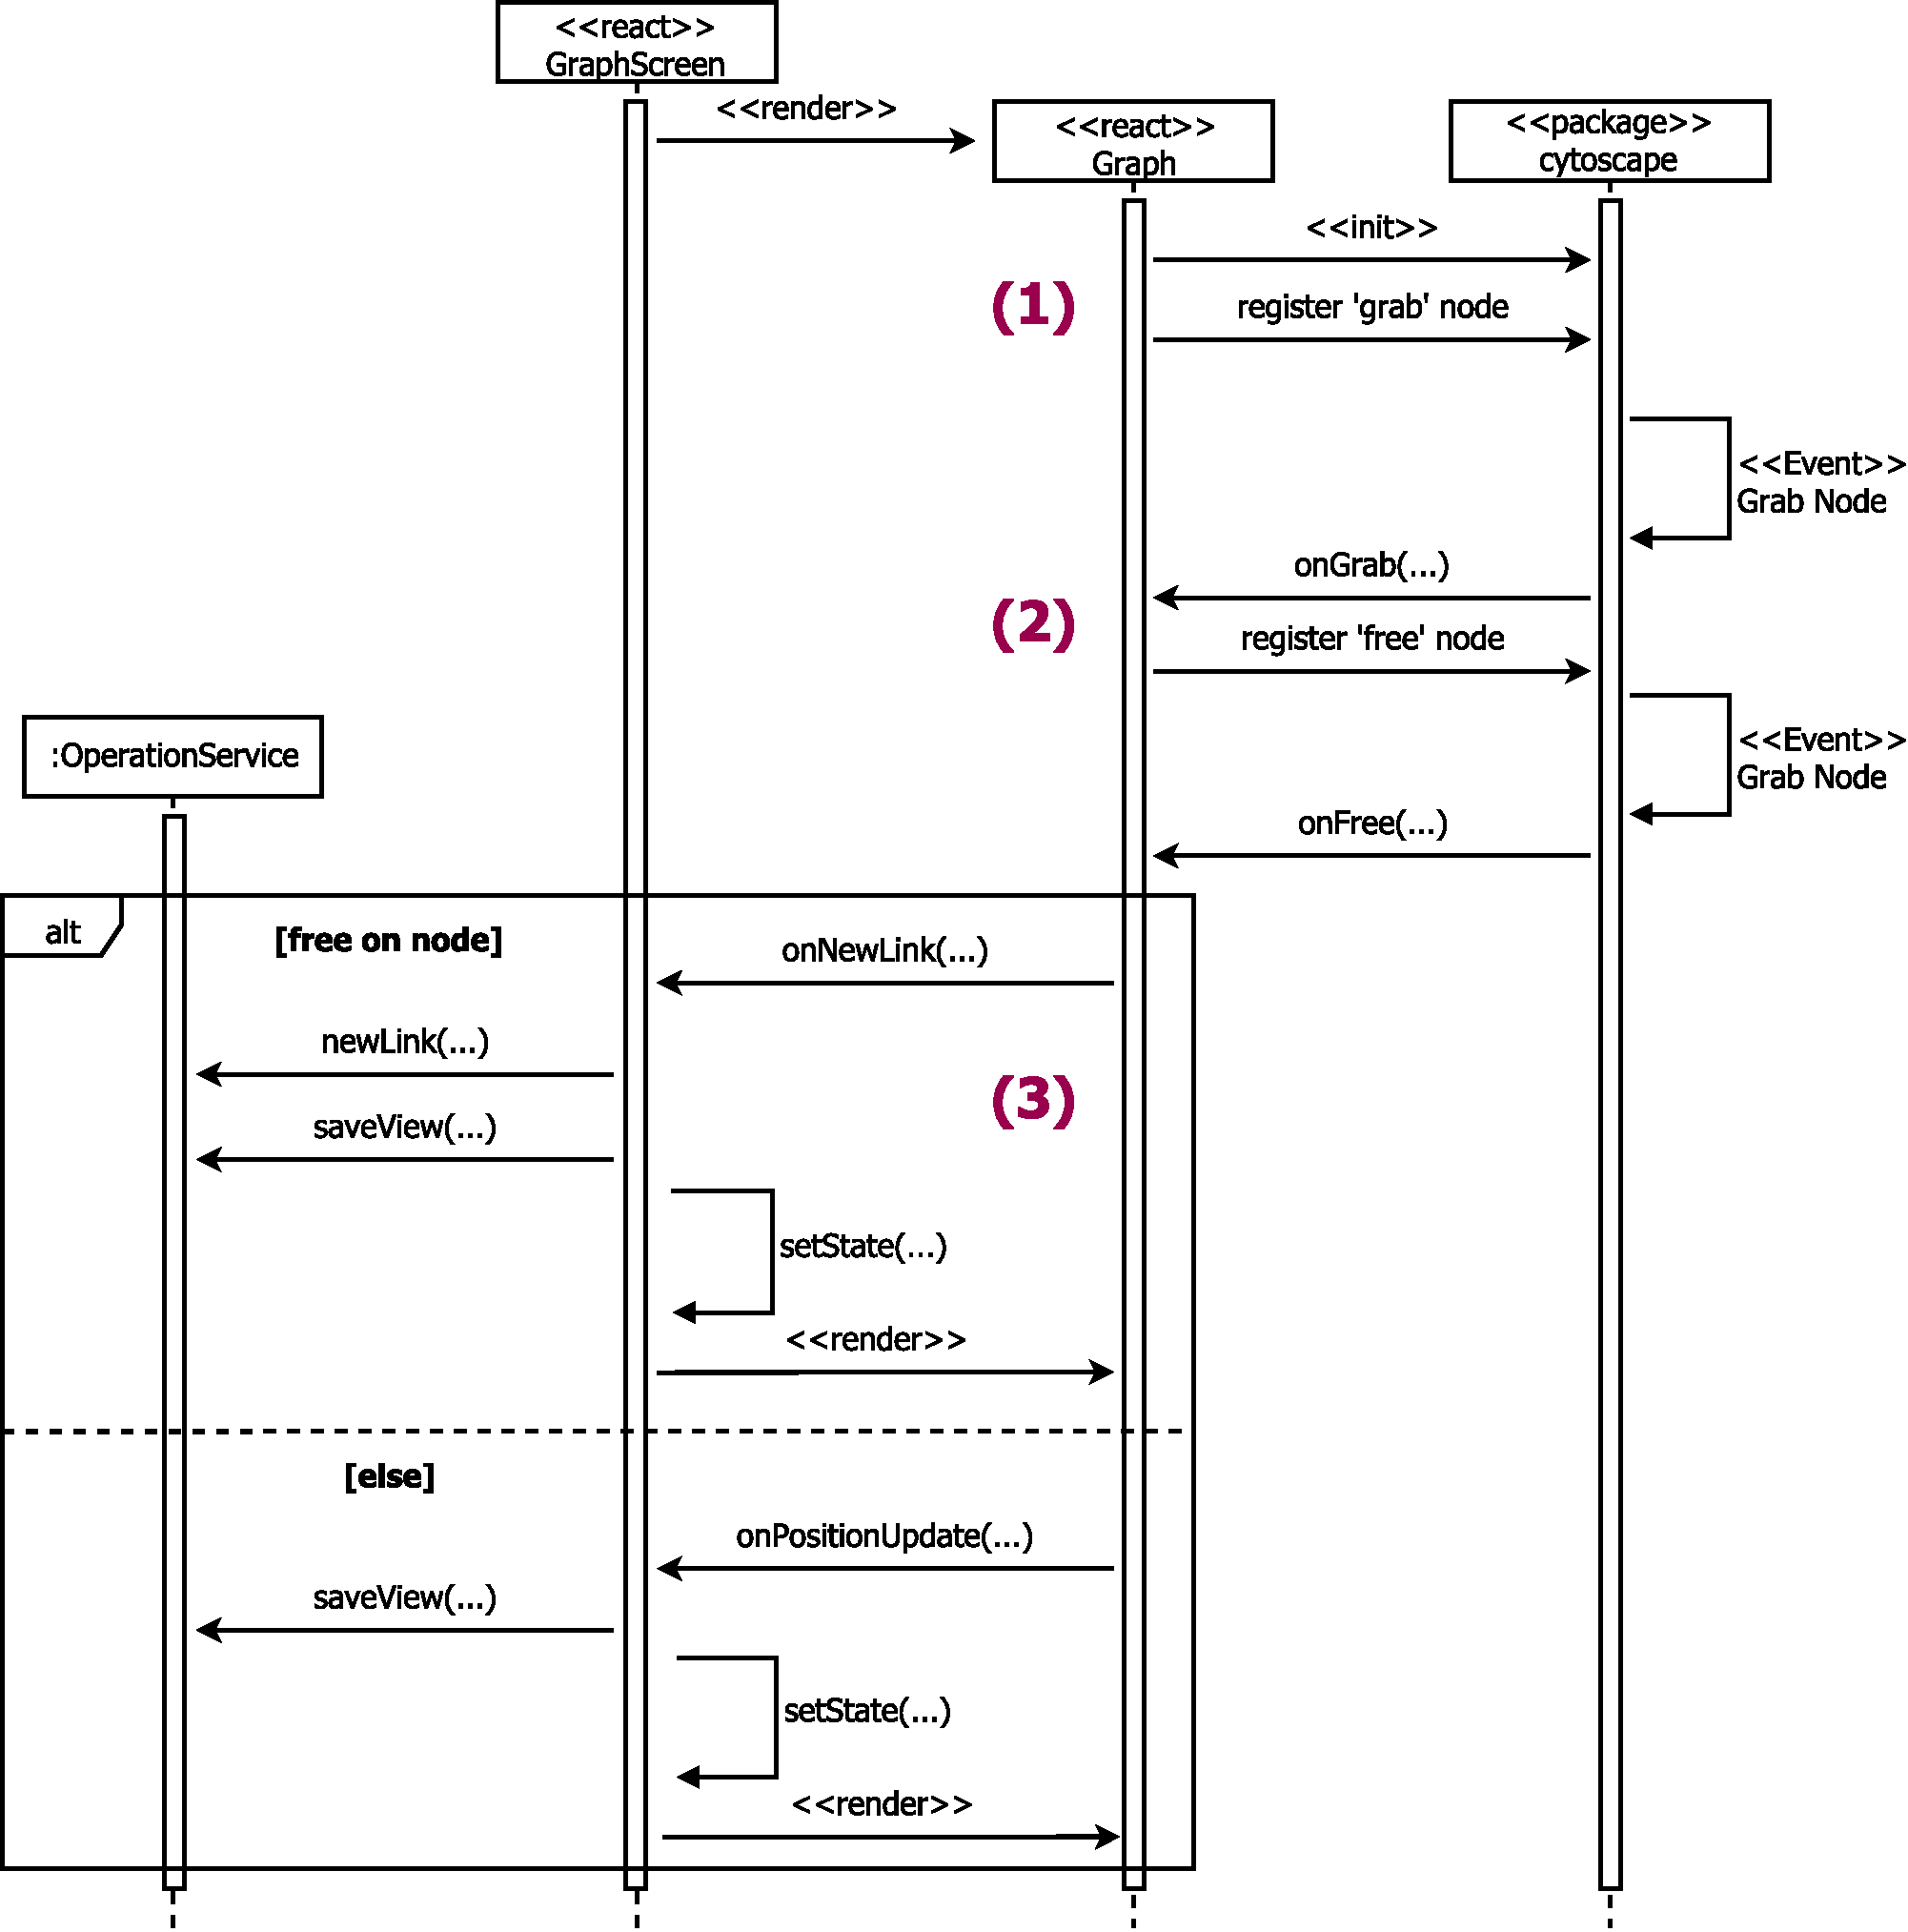
\includegraphics[width=1.2\textwidth]{UpdatePositionDiagramm}}
\caption{Ablauf Update Position / New Link}
\label{fig:sequence-movenode}
\end{figure}

\subsubsection{Add Node/Link To Existing \gls{Node} (Drag'n'Drop)}
Im \autoref{dnd} wurde bereits erläutert, wie ein \gls{Drag'n'Drop} eines \gls{Node}[s] von ausserhalb behandelt wird. Dadurch wird es ermöglicht, die Aktionen \textit{AddNode} und \textit{LinkToExistingNode} per \textit{Drag'n'Drop} auszuführen. Dazu werden weitere Schritte ausgeführt, welche auf diejenigen in der \autoref{fig:dnd-sequence} folgen (\autoref{fig:sequence-afterdrop}):
\begin{enumerate}
    \item Auch bei diesen beiden Aktionen werden zuerst die allgemeinen Schritte abgearbeitet und die Visualisierung als \textit{DropZone} registriert (vgl. \autoref{listing:dnd-handling}).  
    \item Sobald nun ein \gls{Node} über der Visualisierung losgelassen wird, wird die \textit{Graph}-Komponente informiert. 
    \item Anhand der Position des losgelassenen \gls{Node}[s] wird nun ermittelt, ob an dieser Stelle bereits ein \gls{Node} in der Visualisierung dargestellt wird. Falls dies zutrifft, muss der losgelassene \gls{Node} in der Visualisierung dargestellt werden und mit einem \gls{Link} zum \gls{Node} an der losgelassenen Stelle verbunden werden. Dafür sind folgenden Schritte notwendig:
        \begin{itemize}
            \item Mithilfe der entsprechenden \textit{Callback}-Methode wird die \textit{GraphScreen}-Komponente informiert.
            \item Die Änderungen werden nun in der \textit{GraphScreen}-om\-po\-nen\-te ausgeführt und die Datenbasis durch den \hyperref[OperationService]{\textit{OperationService}} informiert.
            \item Durch die Aktualisierung des Zustands der \textit{GraphScreen}-Komponente wird die \texttt{render}-Methode ausgeführt und die Aktualisierungen an die \textit{Graph}-Komponente weitergegeben und somit die Änderungen angezeigt.    
        \end{itemize}
    Wenn nun der \gls{Node} an einer freien Stelle losgelassen wird, soll dieser ohne einen neuen \gls{Link} erstellt werden. Dazu sind folgende Schritte nötig:
        \begin{itemize}
            \item Durch die entsprechenden \textit{Callback}-Methode wird die Information an die \textit{GraphScreen}-Komponente weitergegeben.
            \item Änderungen werden nun innerhalb der \textit{GraphScreen}-Kom\-po\-nen\-te abgearbeitet und die Informationen durch den \hyperref[OperationService]{\textit{OperationService}} an die Datenbasis weitergegeben.
            \item Auch hier wird zum Schluss die Aktualisierung des Zustands der \textit{GraphScreen}-Komponente ausgeführt und somit die \texttt{render}-Methode aufgerufen. Die Aktualisierungen werden an die \textit{Graph}-Komponente weitergegeben und somit die Änderungen angezeigt.    
        \end{itemize}
\end{enumerate}
\begin{figure}[htbp]
\centerline{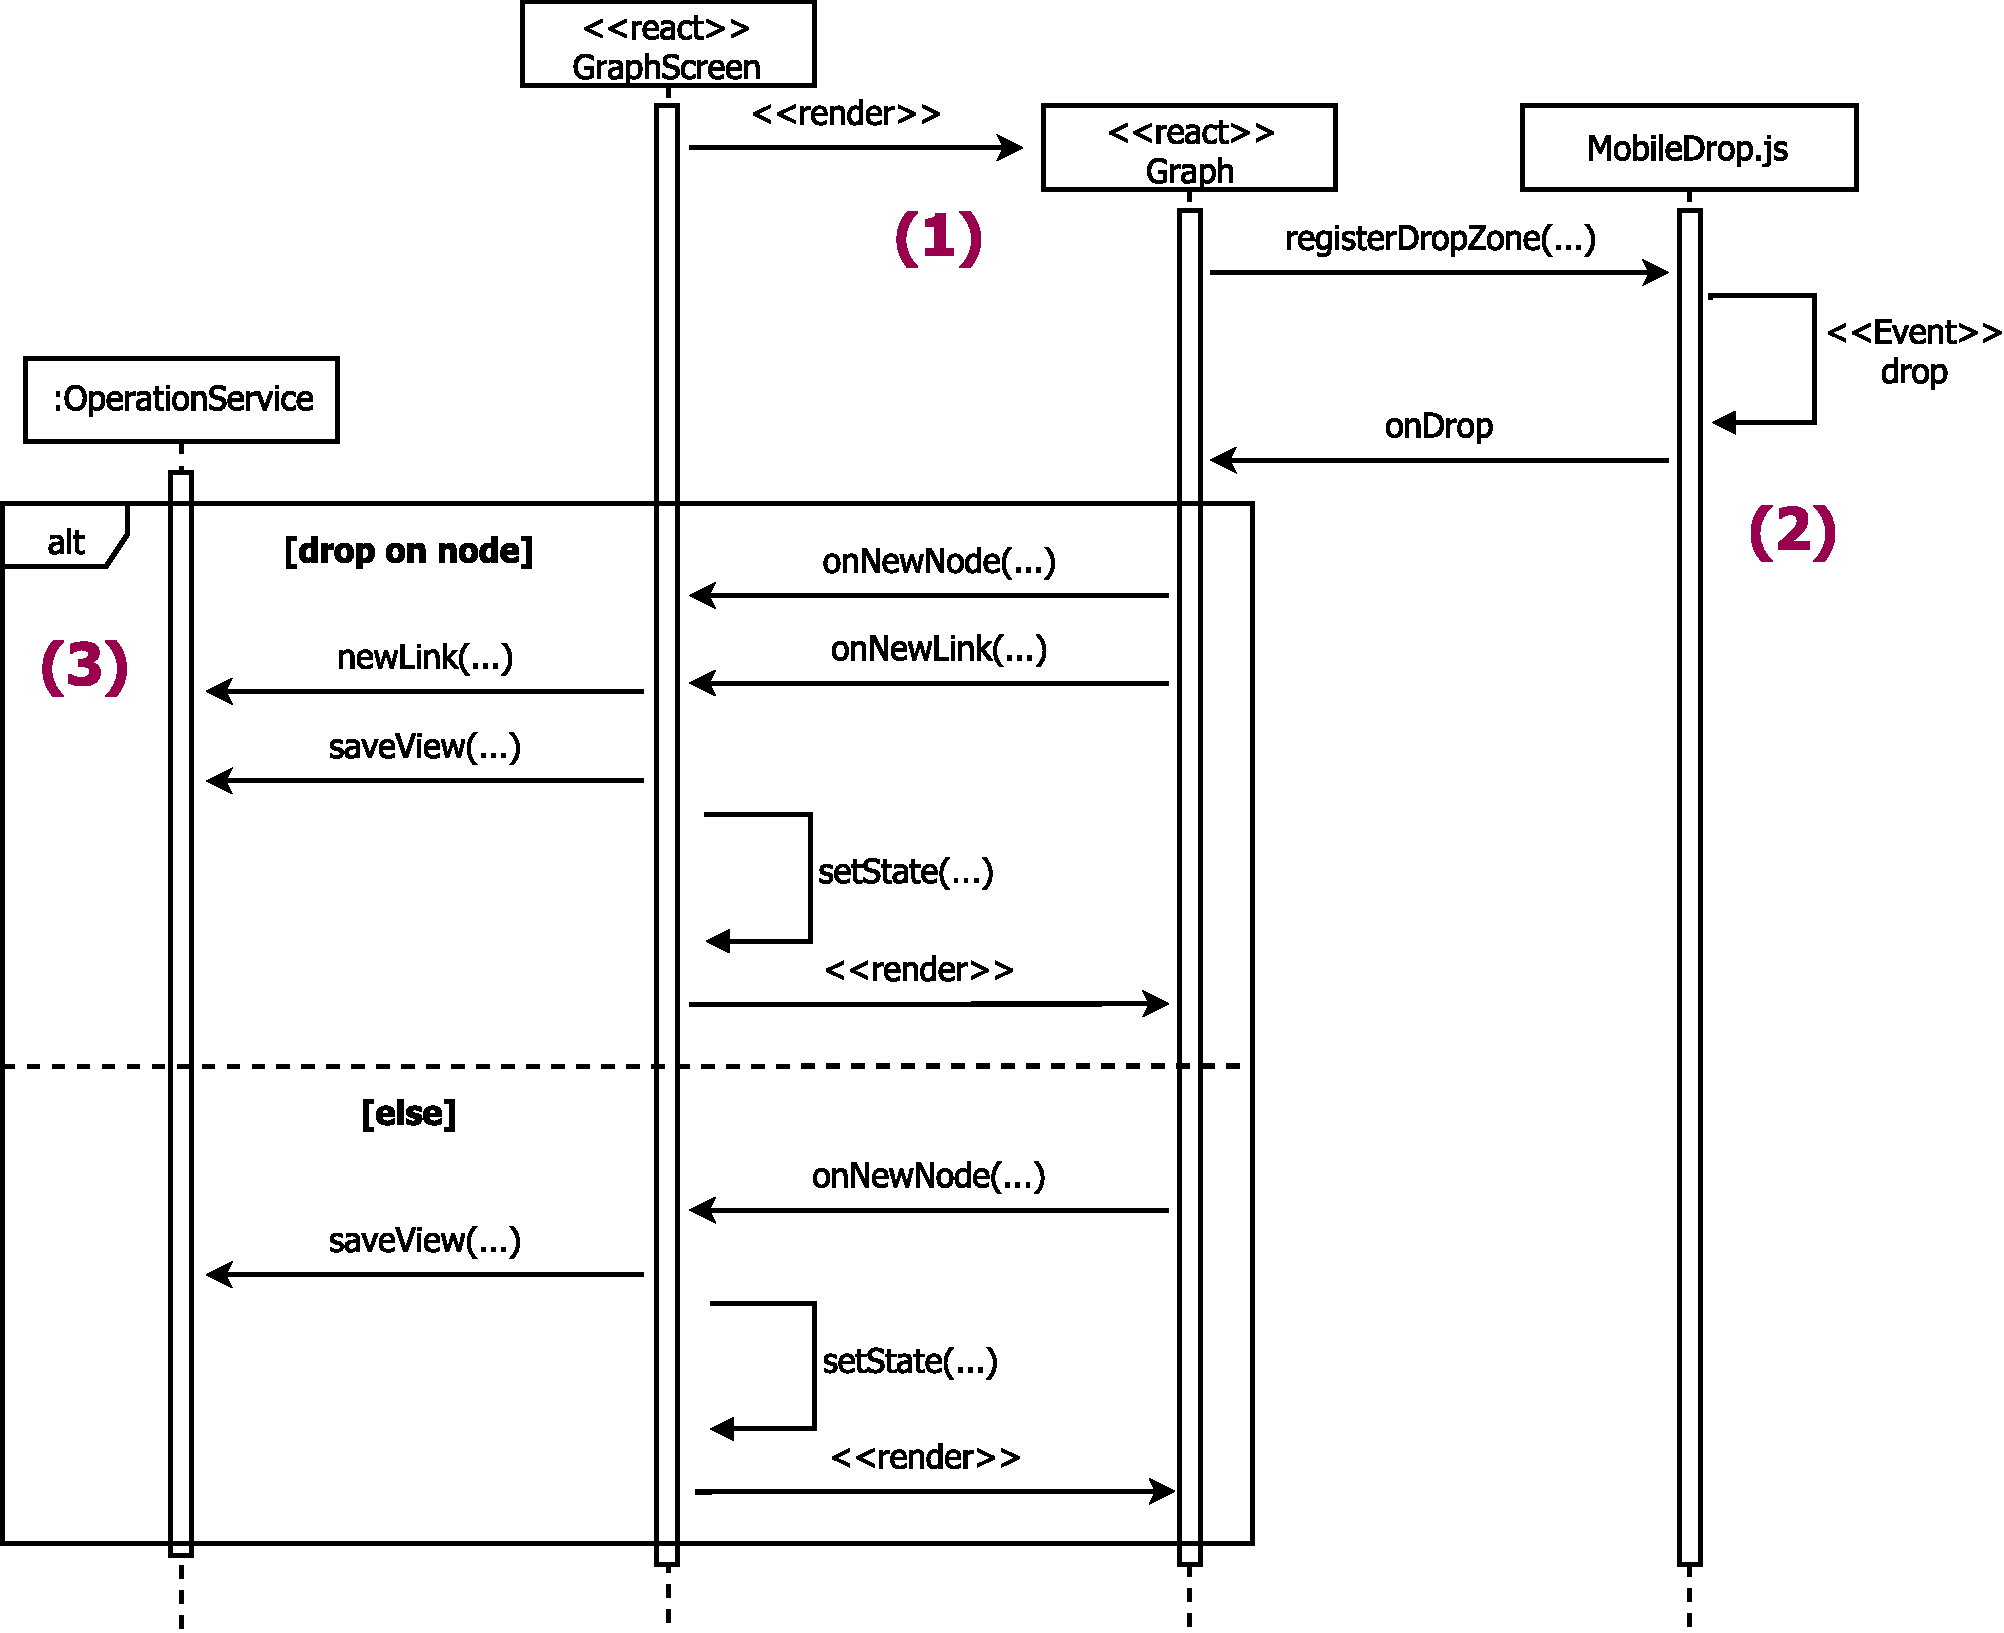
\includegraphics[width=1.2\textwidth]{FurtherProcessDropNode}}
\caption{Ablauf Add Node / Link To Existing Node}
\label{fig:sequence-afterdrop}
\end{figure}


\subsection{Kontextmenüs}
Die beiden Kontextmenüs (\autoref{fig:core-contextmenu} und \autoref{fig:node-contextmenu}) bieten eine Sammlung von \hyperref[subsec:aktionen]{\textit{Aktionen}}, welche der entsprechenden Situation angepasst sind. Beide werden entweder durch einen Rechtsklick (Desktop) oder einen langen Tap (Mobile) aufgerufen. Diese \gls{Event}s werden ebenfalls, wie in \autoref{visual} beschrieben, innerhalb der \textit{Graph}-Komponente beim \textit{cytoscape}-Framework registriert. Sobald der \gls{Event} auftritt werden durch die entsprechenden \textit{Callback}-Methoden die \textit{GraphScreen}-Komponente informiert, damit diese das entsprechende Menü öffnet.

Um die entsprechenden Suchfelder oder Dialoge aufzurufen, nutzen beide Menüs die Implementierung der Schnittstellen \hyperref[SearchFieldFactory]{SearchFieldFactory} oder \hyperref[DialogFactory]{DialogFactory} (\autoref{interaktion}).

\begin{figure}
\centering
\begin{subfigure}[b]{0.5\textwidth}
    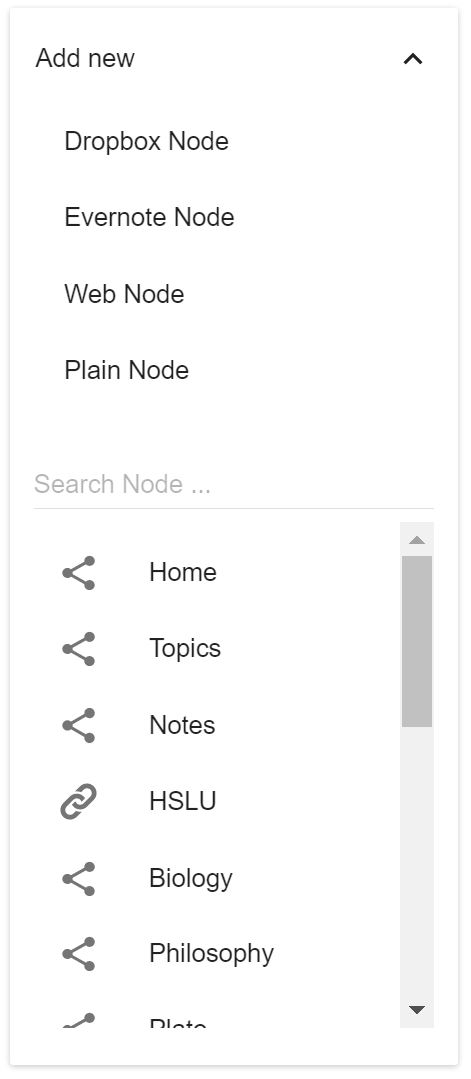
\includegraphics[width=1\linewidth]{CoreContextMenu-Screen}
    \caption{CoreContextMenu}
    \label{fig:core-contextmenu}
    \end{subfigure}
\begin{subfigure}[b]{0.4\textwidth}
    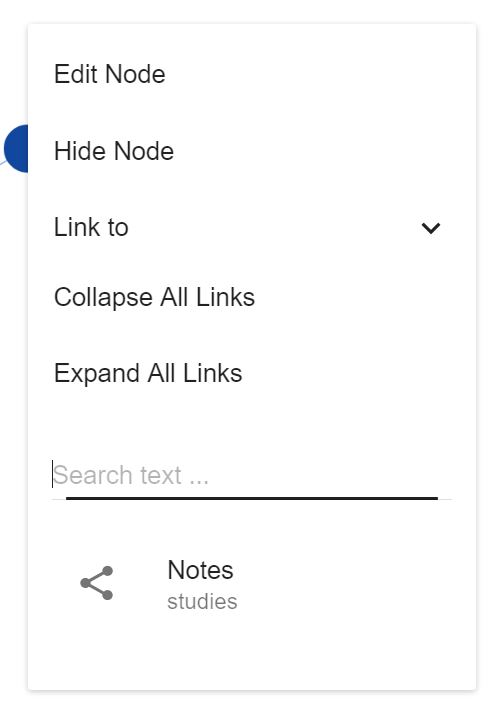
\includegraphics[width=1\linewidth]{NodeContextMenu-Screen}
    \caption{NodeContextMenu}
    \label{fig:node-contextmenu}
    \end{subfigure}
    \caption{Kontextmenüs}
\end{figure}


\subsubsection{CoreContextMenu}
Im \textit{CoreContextMenu} (\autoref{fig:core-contextmenu}) werden die beiden Aktionen \textit{AddNode} und \textit{NewNode} zur Verfügung gestellt (\autoref{subsec:aktionen}). Dabei werden durch die Implementierungen der beiden Schnittstellen \hyperref[SearchFieldFactory]{SearchFieldFactory} und \hyperref[DialogFactory]{DialogFactory} das Suchfeld \textit{GraphNodeSearchField} und der Dialog \textit{NewNodeDialog} bezogen und eingebunden (\autoref{fig:sequence-corecontextmenu}).

\begin{figure}[htbp]
\centerline{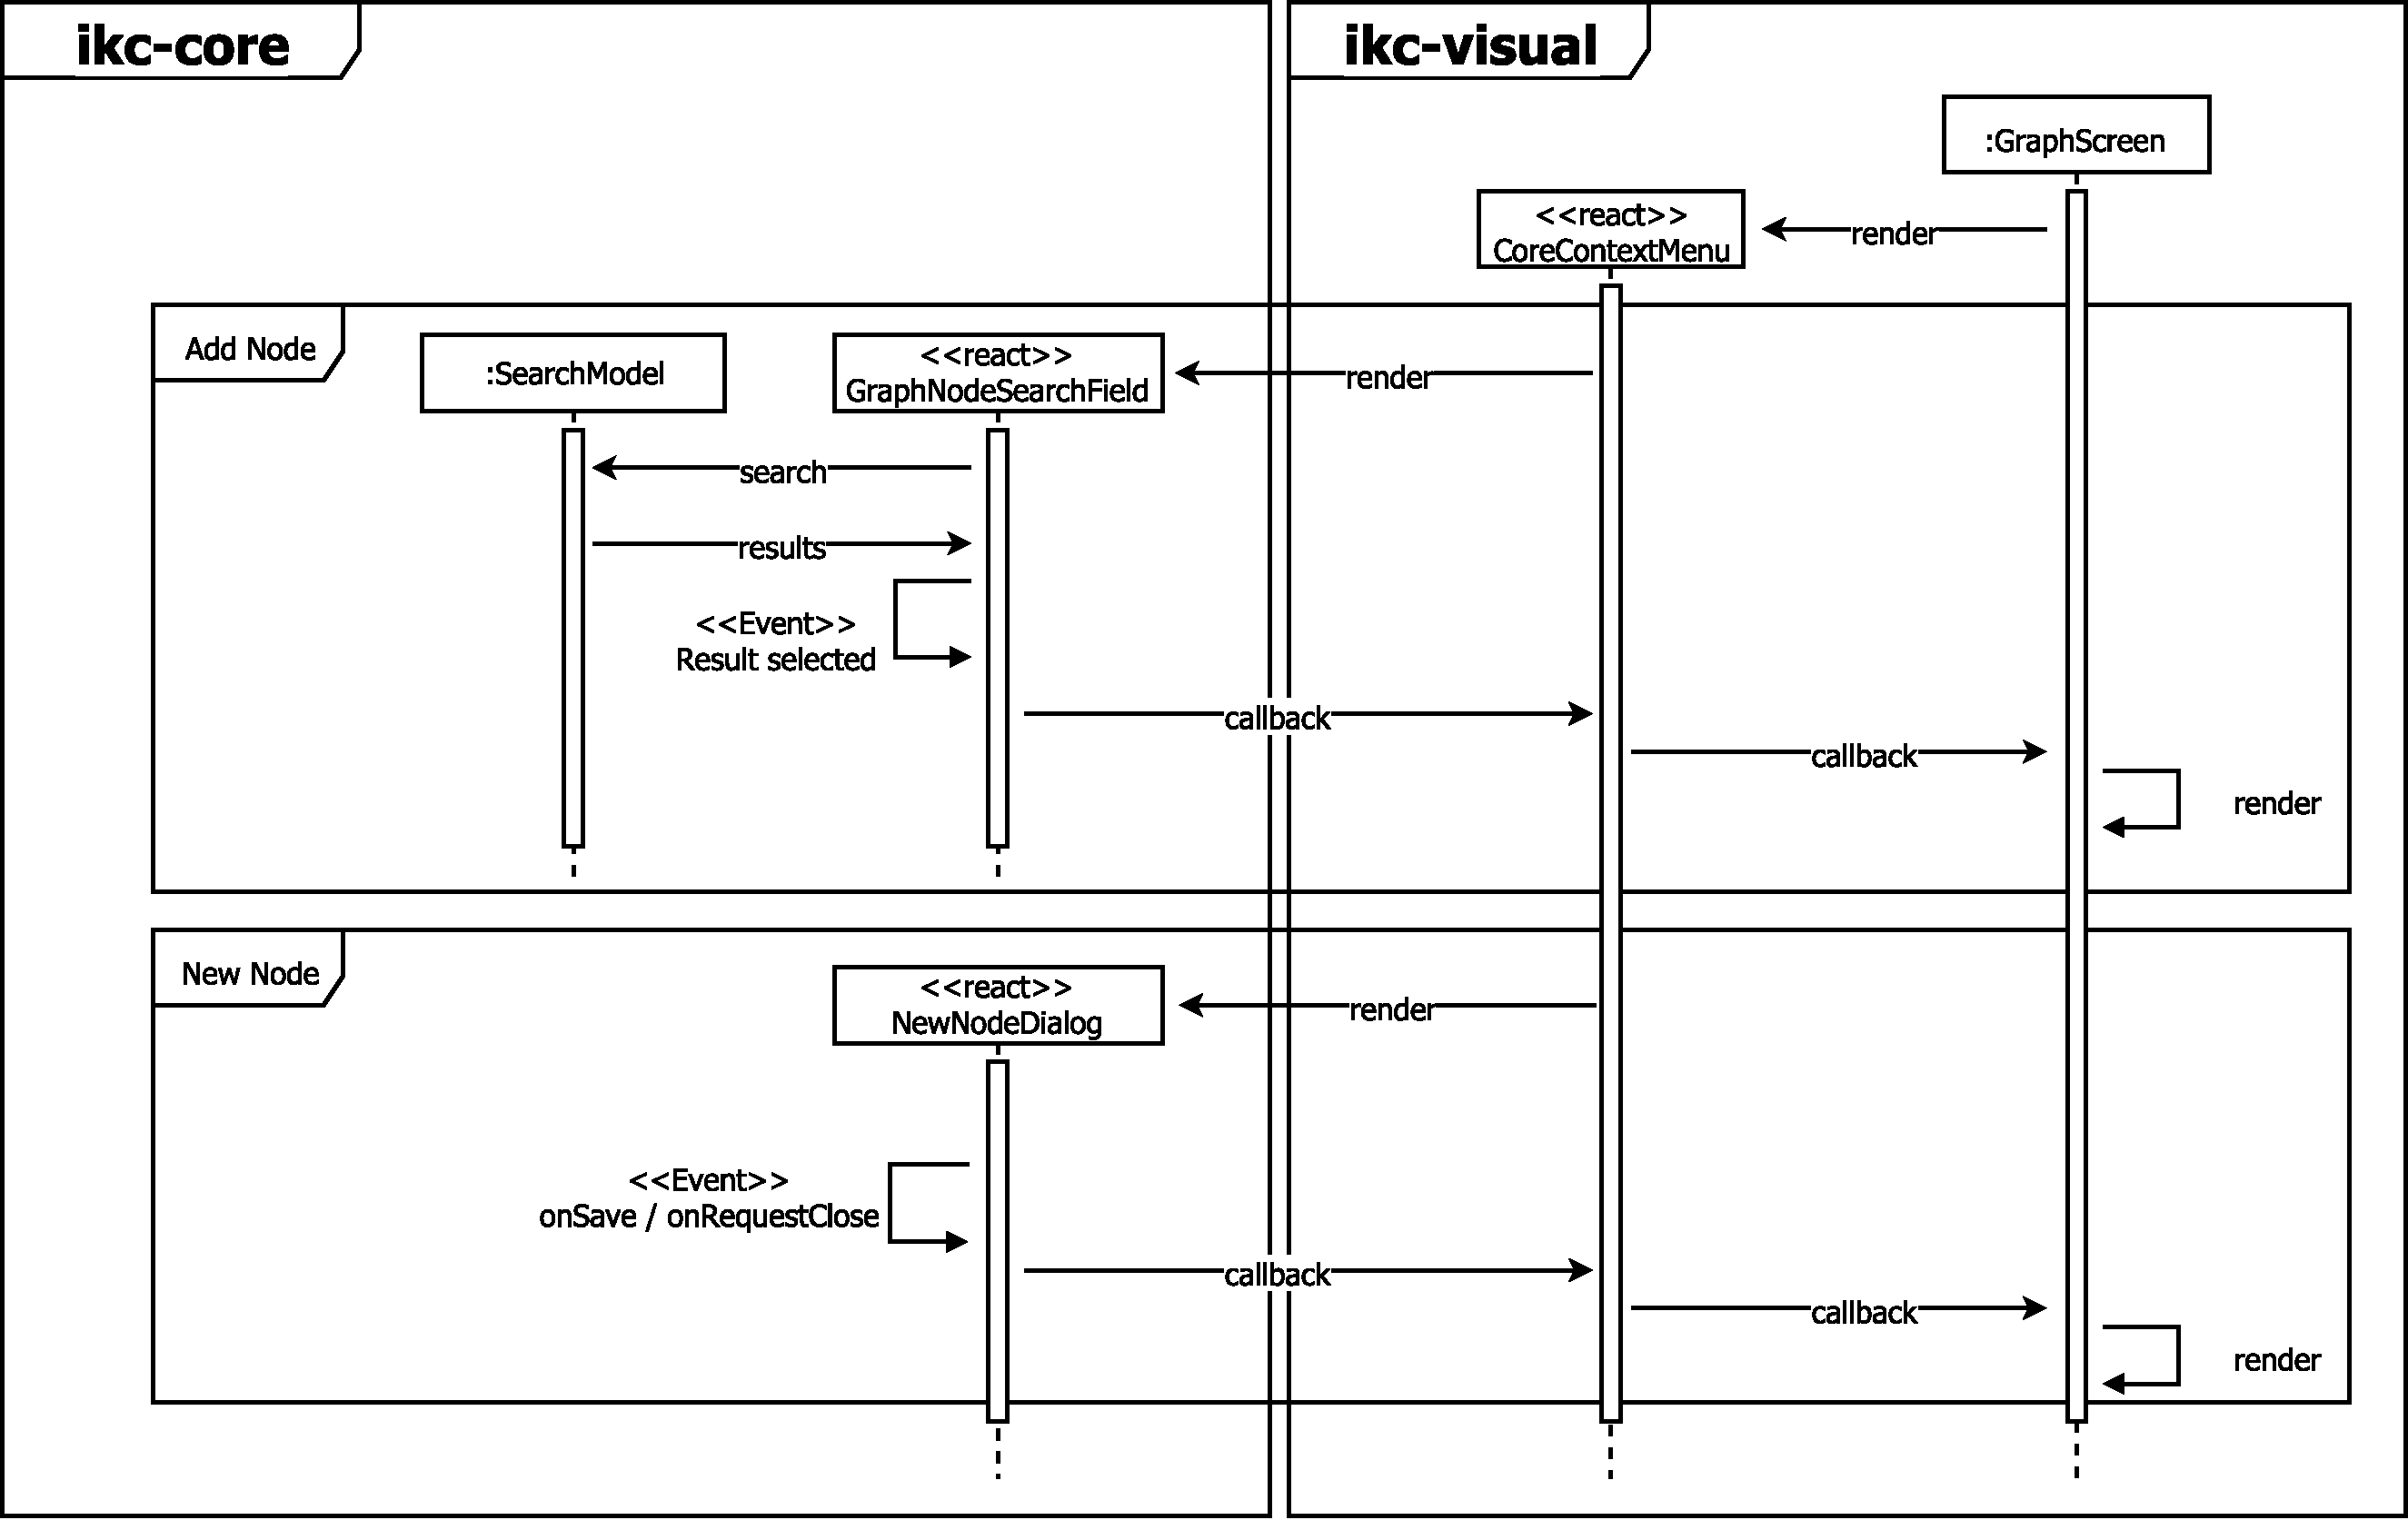
\includegraphics[width=1.2\textwidth]{CoreContextMenuSequence}}
\caption{Ablauf CoreContextMenu}
\label{fig:sequence-corecontextmenu}
\end{figure}


\subsubsection{NodeContextMenu}
Diverse \gls{Node} spezifische Aktionen werden im \textit{CoreContextMenu} zusammengefasst (\autoref{subsec:aktionen}). Dazu werden ebenfalls mithilfe der Implementierungen der beiden Schnittstellen \hyperref[SearchFieldFactory]{SearchFieldFactory} und \hyperref[DialogFactory]{DialogFactory} das Suchfeld \textit{GraphLinkSearchField} und die beiden Dialoge \textit{NewNodeToConnect} und \textit{ExistingNodeToConnect} genutzt (\autoref{fig:sequence-nodecontextmenu}). 
\begin{figure}[htbp]
\centerline{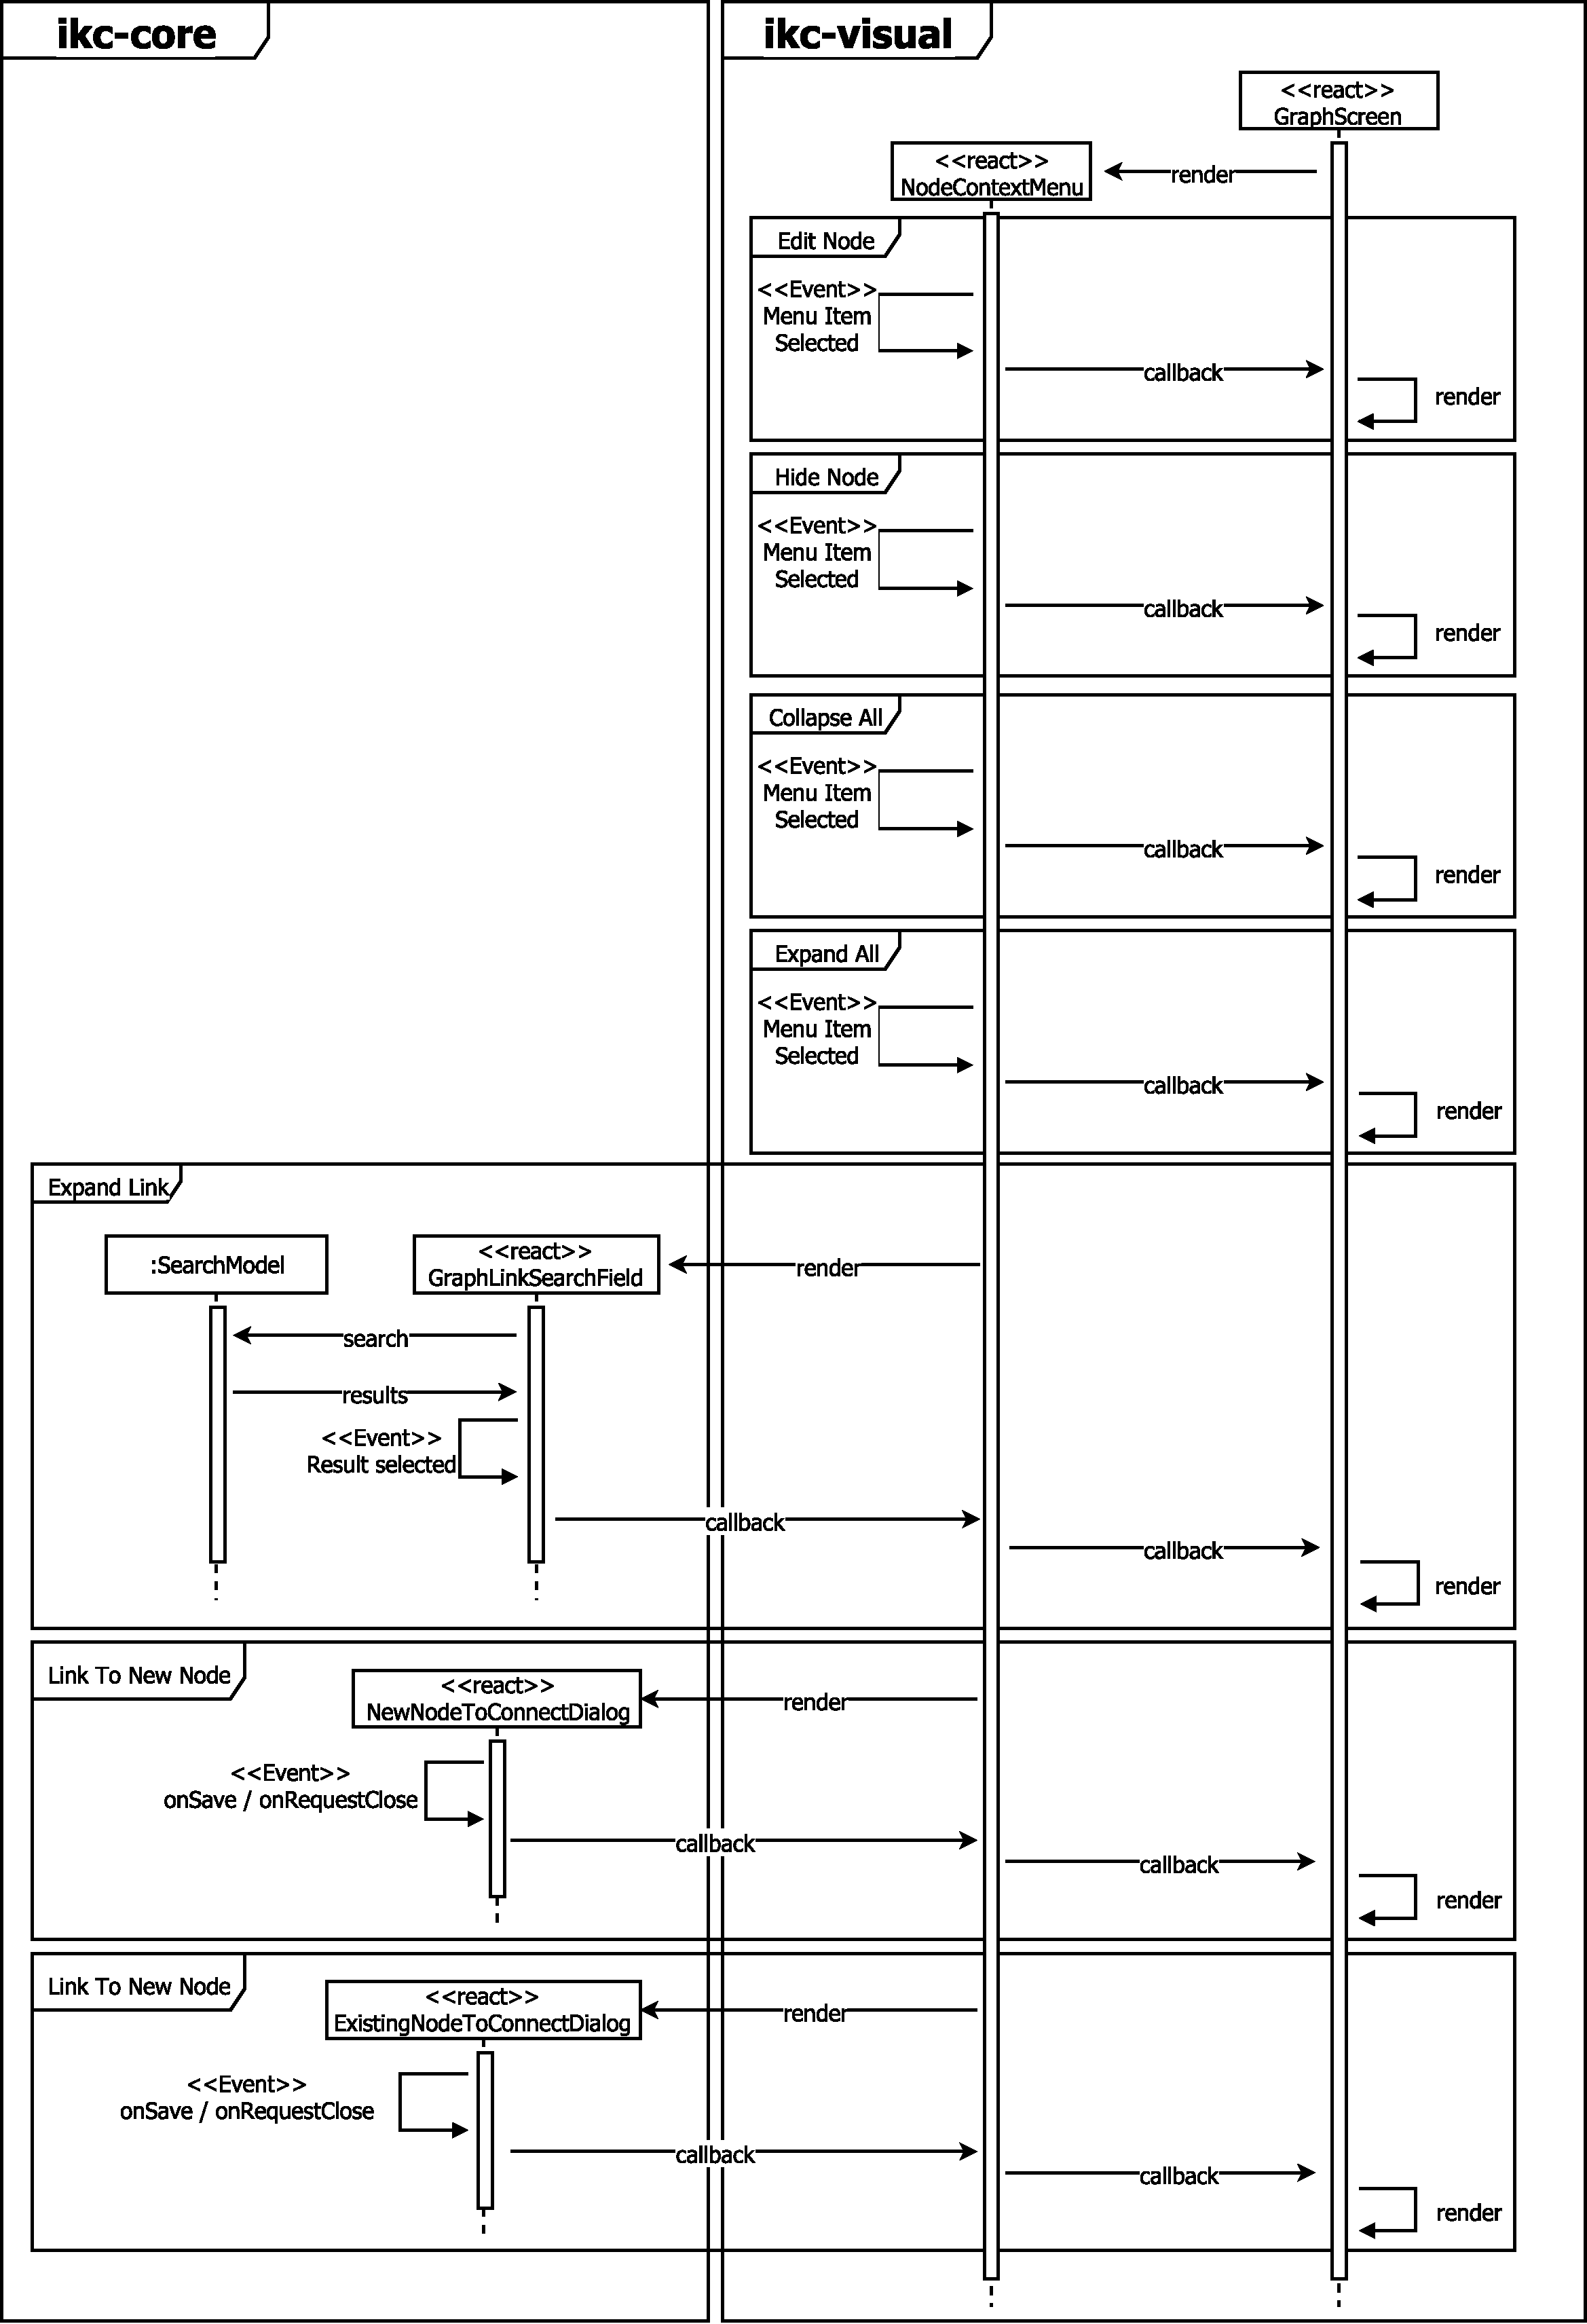
\includegraphics[width=1.15\textwidth]{NodeContextMenuSequence}}
\caption{Ablauf NodeContextMenu}
\label{fig:sequence-nodecontextmenu}
\end{figure}

\section{Integration}
Mit der Integration der Visualisierung in den \textit{ikc-core} wird die Implementation abgeschlossen. Dazu sind die nötigen Schnittstellen zu implementieren und zusätzlich weitere Anpassungen  (\autoref{fig:integration-visualisation}) notwendig:

\begin{itemize}
    \item \textit{GraphVisualisation} - nutzt die \textit{GraphScreen}-Komponente und üb\-er\-gi\-bt ihr alle nötigen Implementationen und Informationen. 
    \item \textit{GraphNodeInformationProvider} - ermöglicht der Visualisierung den Zugriff auf die Datenbasis, um Informationen abzufragen und implementiert die Schnittstelle \hyperref[NodeInformationProvider]{NodeInformationProvider}.
    \item \textit{GraphOperationService} - Dadurch kann die Visualisierung Informationen an die Datenbasis (\textit{NodeService}, \textit{PropertyService} und \textit{ViewService}) weiterleiten. Dazu wird die Schnittstelle \hyperref[OperationService]{OperationService} verwendet.
    \item \textit{GraphDialogFactory} - kapselt die Erstellung der verschiedene Dialog und stellt diese zur Verfügung. Es werden die verschiedenen Methoden der Schnittstelle \hyperref[DialogFactory]{DialogFactory} implementiert.
    \item \textit{GraphSearchFieldFactory} - um die beiden Suchfelder \textit{GraphNodeSearchField} und \textit{GraphLinkSearchField} der Visualisierung zu Ver\-füg\-ung zu stellen, wird die Schnittstelle \hyperref[SearchFieldFactory]{SearchFieldFactory} implementiert.
    \item \textit{ElementIdentityService} - damit die Visualisierung konsistente IDs für neue \gls{Node}[s] und \gls{Link}[s] vergeben kann, werden diese mithilfe der Schnittstelle \hyperref[IdentityService]{IdentityService} implementiert.
    \item \textit{Dialoge} - die verschiedenen Dialoge, welche der Visualisierung durch die \textit{GraphDialogFactory} zu Verfügung gestellt werden, nutzen die \hyperref[subsec:dialoginterfaces]{Dialog-Schnittstellen}. Diese dienen als Grundlage für die \gls{Props}- und \gls{State}-Schnittstellen der \hyperref[react]{\textit{React}}-Komponente.
    \item Um die verschiedenen \gls{View}s strukturiert halten zu können, werden die Klassen \textit{ViewService} und \textit{ViewModel} verwendet. Innerhalb des \textit{ViewModel}s wird auch die Verbindung zur externen Persistierung auf \gls{Dropbox} implementiert.
    \item Bisher wurde die Applikation nach folgendem Schema aufgerufen: \url{https://<host>/node/:node}, wobei \textit{:node} die darzustellende Node-ID enthält, z.B. \url{https://localhost:8888/node/0}. Neu wird das folgende Schema verwendet: \url{https://<host>/:node(/:view)(/:focus)}. Dabei wurden die beiden optionalen Parameter \textit{:view} und \textit{:focus} hinzugefügt. \textit{:view} enthält die entsprechende ID der View, welche darzustellen ist und \textit{:focus} den Wert \textit{node} oder \textit{view} je nachdem, auf welcher Darstellung der Fokus liegt. Dies ist jedoch nur auf der Mobile-Ansicht relevant. Mit dem Aufruf \url{https://localhost:8888/0/0/view} wird der \gls{Node} mit der ID \textit{0} und die Sicht mit der ID \textit{0} geladen, weiter soll der Fokus auf der Visualisierung liegen, falls die Anfrage von einem mobilen Gerät kommt.
    \item Der mobilen Navigationsleiste wurde ein neues Icon hinzugefügt, mit welchem zwischen der Visualisierung und der NodeDetail-Ansicht gewechselt werden kann. 
    \item Für die Navigation in der Mobile- und der Desktop-Ansicht wurde ein neuer Punkt \textit{View} hinzugefügt. Dadurch können neue Views erstellt, bestehende durchsucht und dargestellt werden. Weiter wurde dem Punkt \textit{Delete} zwei Menüpunkte \textit{DeleteView} und \textit{DeleteNode} hinzugefügt. 
    \item Innerhalb des \textit{NodeService} wurden entsprechende Methoden des \textit{ViewService} eingebaut. Somit wird sichergestellt, dass alle Änd\-er\-ung\-en der Datenbasis auch den verschiedenen Sichten weitergegeben werden. So zum Beispiel falls ein \gls{Link} in der Datenbasis gelöscht wird. Diese Änderung muss auch in den Views ausgeführt werden, sodass dieser \gls{Link} nicht mehr dargestellt wird. 
    
\end{itemize}

\begin{figure}[htbp]
\centerline{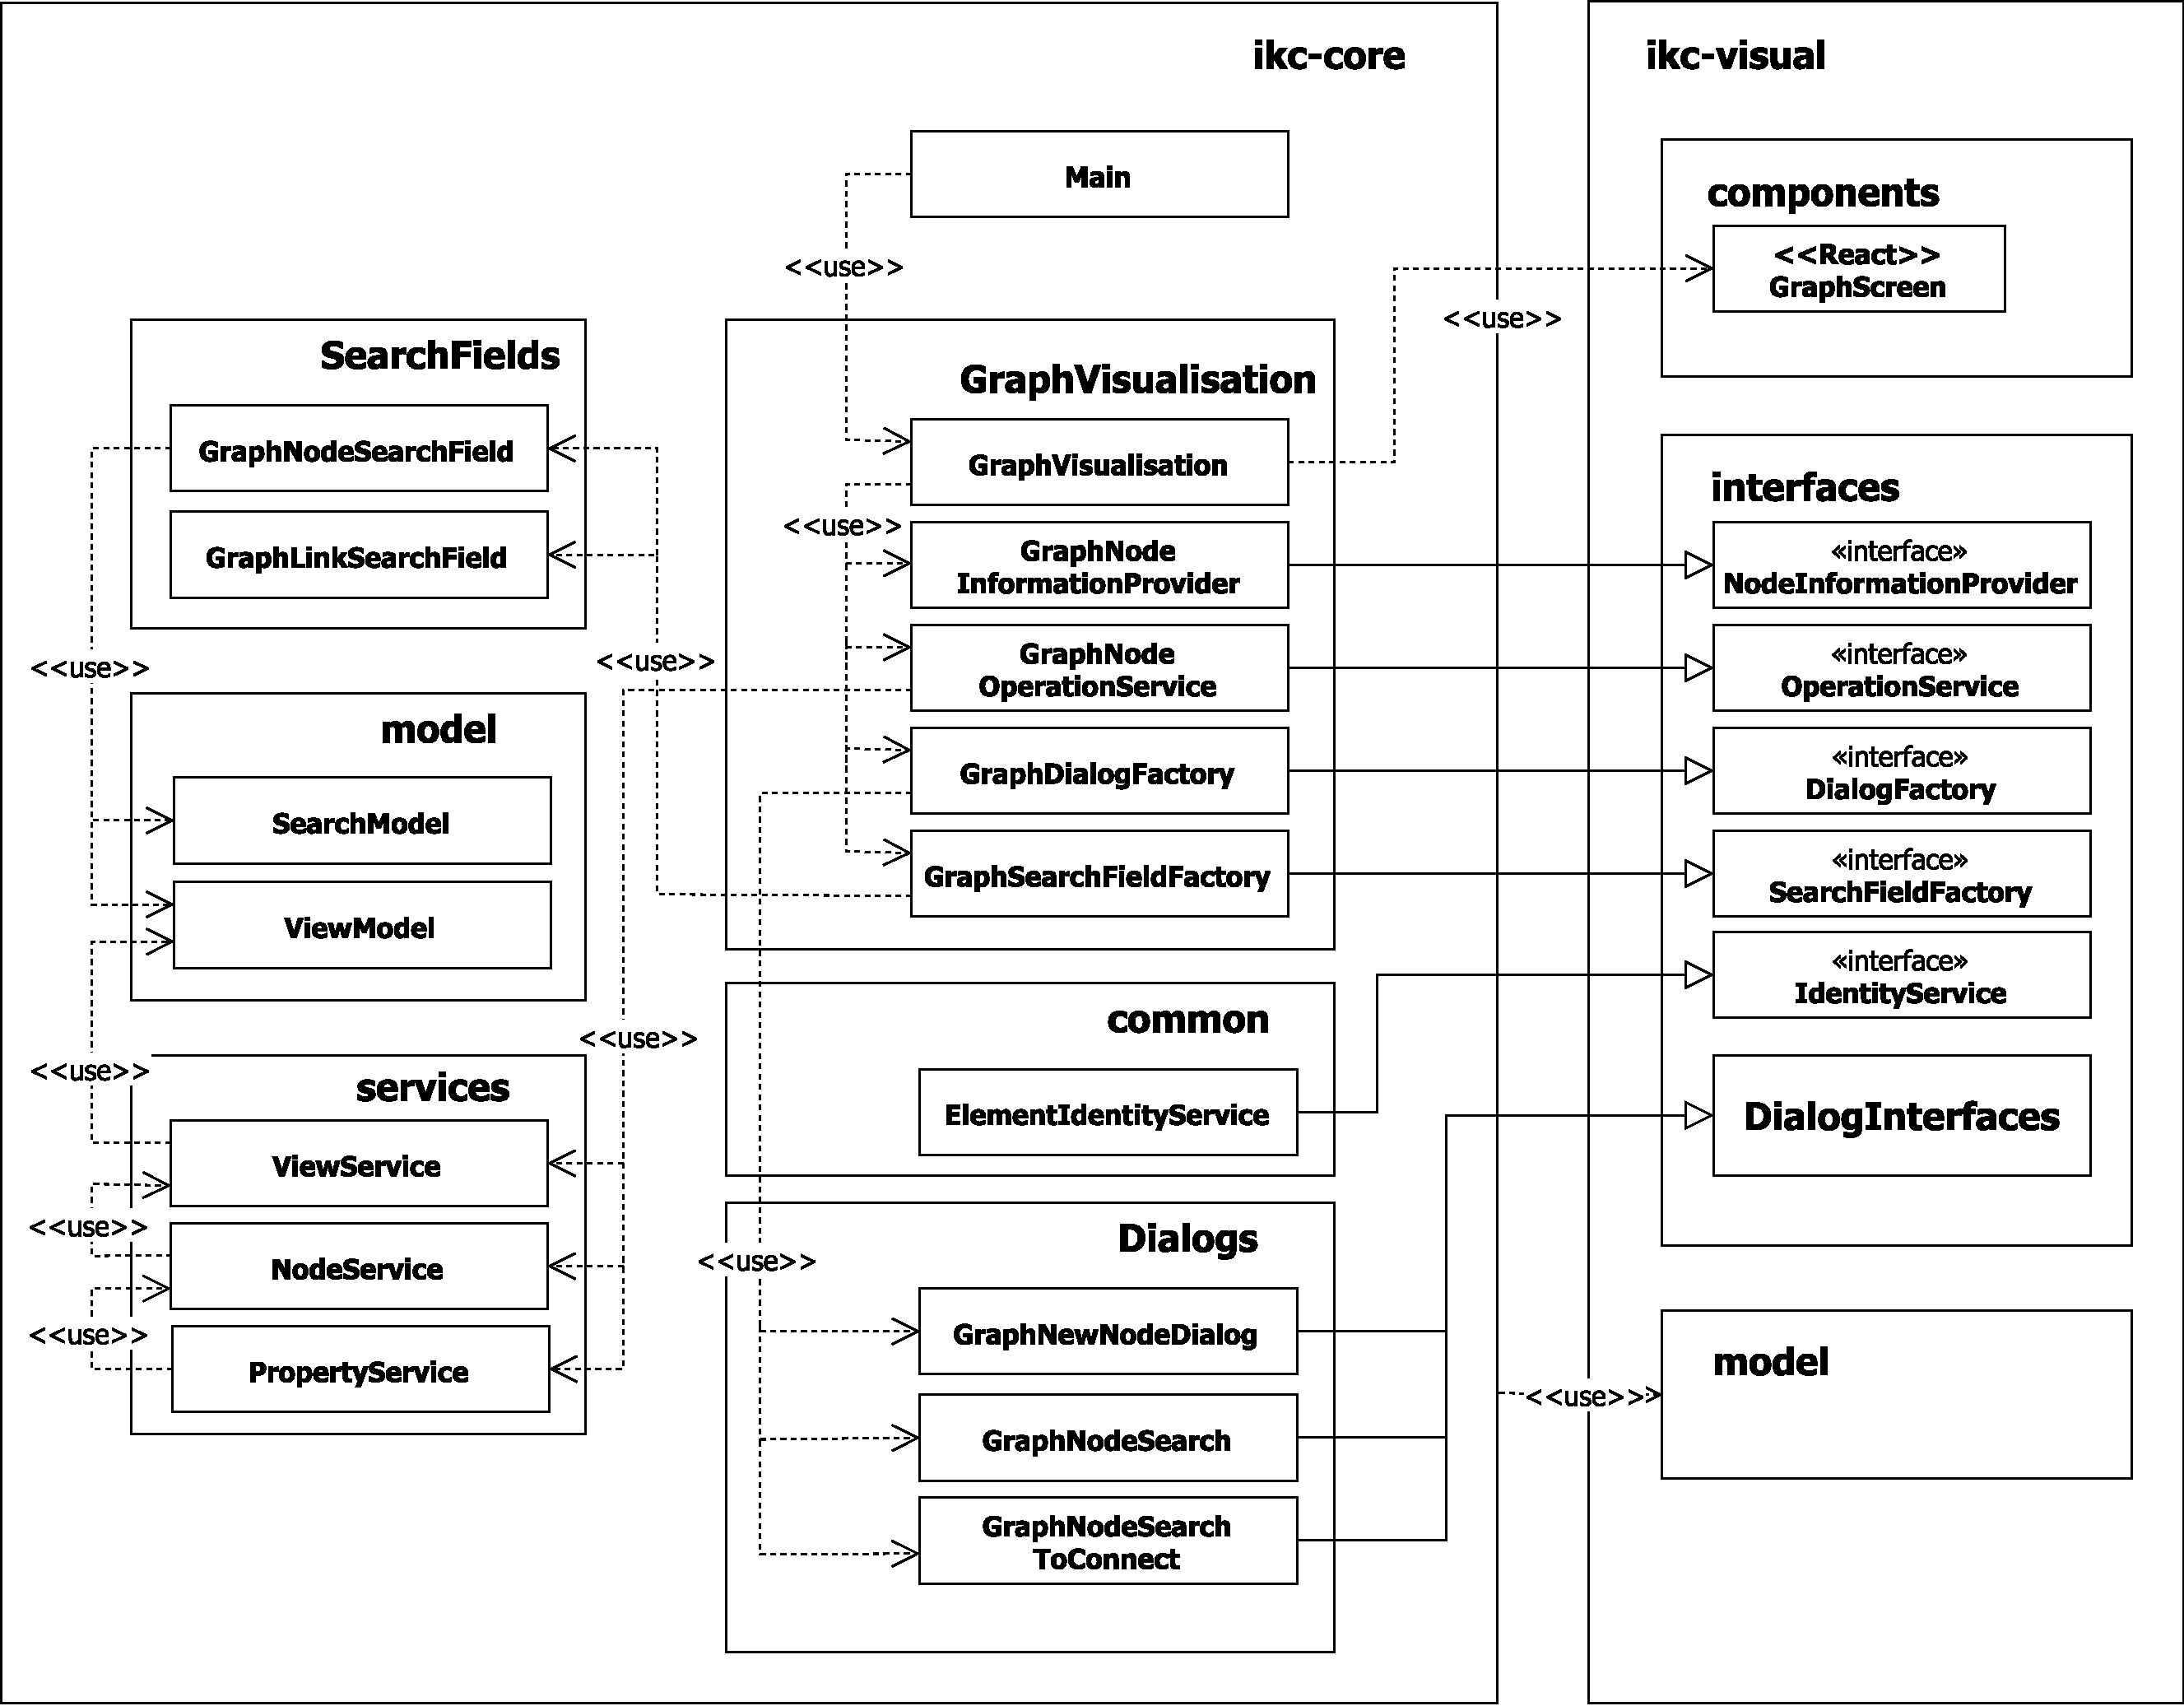
\includegraphics[width=1.3\textwidth]{ikc-visual-integration}}
\caption{Intergration Visualisierung}
\label{fig:integration-visualisation}
\end{figure}

